



\chapter {BALANCE}
\label{cha:cont1}
 In this chapter, I describe my contributions to the BALANCE project. 

\section{Introduction}

The bioengineering approaches for lifestyle activity
and nutrition continuous engagement (BALANCE) project was a multi-year, interdisciplinary project with the goal of designing, building, and evaluating a mobile-phone based application to help people overcome these challenges of tracking their overall balance of energy intake and expenditure. It combines a wearable device that calculates caloric expenditure with a mobile phone that includes a food diary to track caloric intake. The software also includes a visualization that reports the real-time energy balance for the day. The wearable device is built using the multi-sensor board (MSB) \citep{lester_validated_2009}. The MSB contains an accelerometer, now standard in mobile phones, as well as other sensors that aide in physical activity detection.  

The software consists of three main components: a ``fuel gauge'' visualization that reflects the current caloric balance; a food diary; and a physical activity diary. The food diary requires users to enter the details of what they eat, while the physical activity diary accepts input from the external MSB device that calculates most calories burned from physical activity (the exception being water or high-impact sports, which need to be manually entered).
 
\subsection{Project Overview}
Many people were involved in this multi-phase project. The project included brainstorming designs for and evaluation of the fuel-gauge visualization; running a paper prototype evaluation of the software based on specified need, goals and reviews of similar tools; building an initial prototype on a feature phone platform; validating the algorithms on the MSB for calculating calorie expenditure; and executing an iterative design and implementation process of the application on a smartphone. Finally, we combined the smartphone software and MSB validated the system overall. My primary contribution to this project was the design and implementation of the smartphone software. The rest of this chapter describes the process and final product in further detail. 

Multiple documents describe contributions to the BALANCE project. Tamara Denning contributed to the initial design and paper prototype evaluations \citep{denning_balance:_2009}. Deonna Hughes designed, conducted, and analyzed the focus groups and prototype iterations \citep{hughes_balance:_2009}. She looked at two metrics for improvement from iteration to iteration. The first was the result of standardized usability questionnaires; the other was the time between when participants ate a food and when they entered it in the diary. Neither metric showed significant improvement in the prototype over 5 iterations. I discuss this in further detail later in this chapter. Jonathan Lester designed and evaluated the calorie expenditure algorithms \citep{lester_validated_2009}, employing a gold-standard oxygen-consumption evaluation methodology. Algorithms using the MSB sensor data were 89.54\% (+/- 7.25\%) accurate in the lab and 79.8\% (+/- 9.48\%) in the field.  Heather Snively designed and conducted the overall system validation \citep{snively_balance_2010}. Participants used the entire system for 4 days, tracking their food intake on days 1, 3, and 4. On day 2 participants provided a 24-hr recall of what they ate on day 1, which was compared to entries in the food diary on the first day. The average percent calorie difference between the mobile phone food diary and the 24-hr recall was 9 +/- 18\%.  

\section{Fuel-Gauge Visualization}
The goal of the BALANCE project was to combine a food diary to collect information about energy intake, a physical activity component (diary + MSB) to collect energy expenditure information, and the fuel gauge visualization to show the current energy balance throughout the day. The heart of the system was a unifying user interface on a mobile phone. 

The first investigation focused on the fuel-gauge visualization. The visualization needed to provide the current overall energy balance, but it was unclear what other information would be necessary or relevant. Additionally, the visualization needed to be understandable at a glance, provide more meaning upon reflection, and work within the constraints of the target device in terms of size and resolution. One concern was the level of abstraction: whether the visualization depicts a concrete, physical world phenomena or a more mathematically-oriented graph view. In this section, I describe a lab-based paper prototype user study to collect feedback on a wide range of potential visualizations. Results informed the design decisions for the BALANCE prototypes. 

\subsection{Participants}
12 participants (10 female and 2 male) were recruited from a university community. Ages ranged from 18-50, with a majority (8) in the 30-40 year age range. 

\subsection{Procedure}
After providing written informed consent, participants completed a survey collecting basic demographic information. Participants rated the desirability of given features for food and exercise applications on a mobile phone, then discussed what they had eaten that day (or the previous day, depending on time of interview), including context (what they ate, how much, where, when, and how much that meal varies for them). 

Next, participants were shown the different visualizations. Each visualization depicted the same four situations: the start of the day, before any food is entered or calories expended; the end of the day, when more than the day's goal had been consumed and expended; and two points in between, showing various balance levels. \textbf{REVISIT THIS. It's not true. } Figure \ref{fig:viz1series} shows one of the visualizations in each energy balance example. 


\begin{figure}[tbh]
	\centering
	\begin{subfigure}[t]{1.25in}
		\centering
		\setlength\fboxsep{0pt}
\setlength\fboxrule{0.5pt}
\fbox{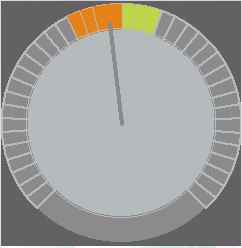
\includegraphics[width=1.25in]{./images/cont1/Viz_1_1}}
		\caption{Shows a day with a small breakfast early in the day. }\label{fig:viz1_1}
	\end{subfigure}
\quad
	\begin{subfigure}[t]{1.25in}
		\centering
		\setlength\fboxsep{0pt}
\setlength\fboxrule{0.5pt}
\fbox{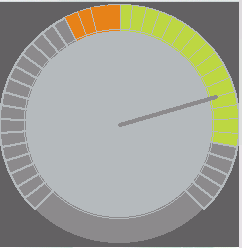
\includegraphics[width=1.25in]{./images/cont1/Viz_1_2}}
		\caption{Shows a day when the user ate a large breakfast. }\label{fig:viz1_2}
	\end{subfigure}
\quad
	\begin{subfigure}[t]{1.25in}
		\centering
		\setlength\fboxsep{0pt}
\setlength\fboxrule{0.5pt}
\fbox{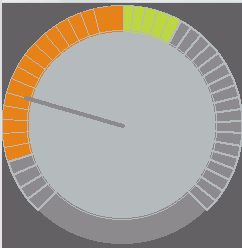
\includegraphics[width=1.25in]{./images/cont1/Viz_1_3}}
		\caption{Represents a day with more exercise early in the day, and some food eaten.}\label{fig:viz1_3}
	\end{subfigure}
\quad
	\begin{subfigure}[t]{1.25in}
		\centering
		\setlength\fboxsep{0pt}
\setlength\fboxrule{0.5pt}
\fbox{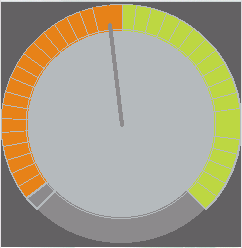
\includegraphics[width=1.25in]{./images/cont1/Viz_1_4}}
		\caption{An end-of-day state, near balance. Both targets are almost met. }\label{fig:viz1_4}
	\end{subfigure}
\quad
	\begin{subfigure}[t]{1.25in}
		\centering
		\setlength\fboxsep{0pt}
\setlength\fboxrule{0.5pt}
\fbox{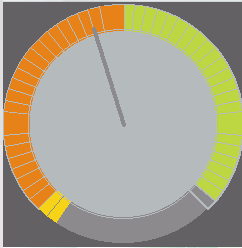
\includegraphics[width=1.25in]{./images/cont1/Viz_1_10}}
		\caption{A near-balance, end-of-day state. Exercise target was surpassed, and food intake was not yet met.}\label{fig:viz1_5}
	\end{subfigure}
\quad
	\begin{subfigure}[t]{1.25in}
		\centering
		\setlength\fboxsep{0pt}
\setlength\fboxrule{0.5pt}
\fbox{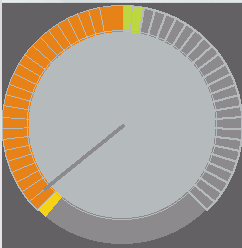
\includegraphics[width=1.25in]{./images/cont1/Viz_1_12}}
		\caption{Lots of exercise, little food eaten.}\label{fig:viz1_6}
	\end{subfigure}

	\caption{Visualizations with various energy intake and expenditure values. }\label{fig:viz1series}
\end{figure}

\begin{figure}

\end{figure}

There were two categories: graphs (two total) and visualizations (five total). Participants were asked to rank their preferred visualizations within each category and offer comments. 

\subsection{Instruments}
The team brainstormed seven candidate visualizations. The features of different visualization concepts included abstract versus concrete metaphors; a single balance indicator (energy balance is more intake or more expenditure); the amount of both energy intake and expenditure as well as overview; how each amount and the balance changes over time; and whether to include an affective component. Previous work investigates the value of having abstract versus concrete representations [ref], so we aimed for a wide range at this point in the design process. 

We adopted an overall simplifying construct for calorie counting called ``CHIPs'': counting hundreds impact point (\citep{beresford_worksite_2007}). A CHIP is simply a unit of 100 calories. Experts involved in the project noted previous success with this simplification. In their previous experience, participants in a workplace wellness program found the CHIP simplification easier to count and keep track of larger increments (smaller numbers). In the BALANCE software, all calorie counts are reported in CHIPs, both for intake and expenditure.  

The main goal of the visualization is to depict the current energy intake/expenditure balance. Other pieces of information that could be helpful included: 
\begin{enumerate*}
\item Goal calorie expenditure and intake for a current day;
\item Progress toward that goal/target over the course of the day; and
\item Whether or how much the user was over the intake or expenditure goal for the day. 
\end{enumerate*}

Mobile phone displays vary greatly in their capabilities, specifically in size and resolution. We used Python for S60 to prototype the visualizations on the target mobile phone, saved them as screenshots, then printed them on paper. This allowed us to present a psuedo-realistic rendering of the visualizations to users. The study artifacts needed to reflect the detail of the visualization within the constraints of the display, as well as the early design stage. Presenting the visualizations on the actual mobile device could raise user
 expectations of the visualization, while paper prototypes and screenshots help to restrain user expectations appropriately. The visualizations were deliberately ``rough'' and unrefined, to target the level of refinement ideal for a paper prototype. 

\begin{figure}[tbh]
	\centering
	\begin{subfigure}[t]{1.25in}
		\centering
		\setlength\fboxsep{0pt}
\setlength\fboxrule{0.5pt}
\fbox{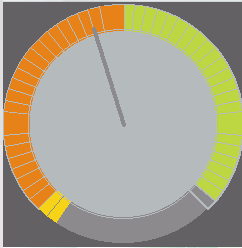
\includegraphics[width=1.25in]{./images/cont1/Viz_1_10}}
		\caption{\textbf{Viz1.} A combination bar graph and fuel gauge-style visualization. }\label{fig:viz1}
	\end{subfigure}
\quad
	\begin{subfigure}[t]{1.25in}
		\centering
		\setlength\fboxsep{0pt}
\setlength\fboxrule{0.5pt}
\fbox{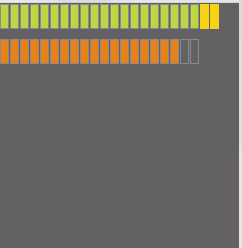
\includegraphics[width=1.25in]{./images/cont1/Viz_2_5}}
		\caption{\textbf{Viz2.} A bar graph style, requires minimal space.}\label{fig:viz2}
	\end{subfigure}
\quad
	\begin{subfigure}[t]{1.25in}
		\centering
		\setlength\fboxsep{0pt}
\setlength\fboxrule{0.5pt}
\fbox{
\includegraphics[width=1.25in]{./images/cont1/Viz_3_3}}
		\caption{\textbf{Viz3.} A simple fuel gauge visualization. The position of the needle and the color of the background indicate balance.}\label{fig:viz3}
	\end{subfigure}
\quad
	\begin{subfigure}[t]{1.25in}
		\centering
		\setlength\fboxsep{0pt}
\setlength\fboxrule{0.5pt}
\fbox{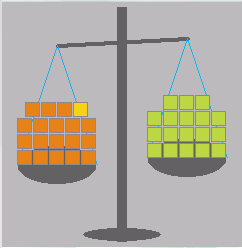
\includegraphics[width=1.25in]{./images/cont1/Viz_4_4}}
		\caption{\textbf{Viz4.} A physical metaphor of a balance scale. Each CHIP is represented by a block. }\label{fig:viz4}
	\end{subfigure}
\quad
	\begin{subfigure}[t]{1.25in}
		\centering
		\setlength\fboxsep{0pt}
\setlength\fboxrule{0.5pt}
\fbox{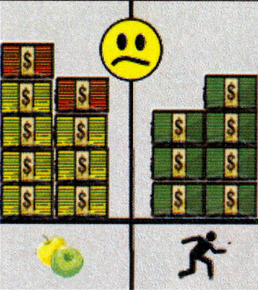
\includegraphics[width=1.25in]{./images/cont1/money}}
		\caption{\textbf{Viz5.} This visualization incorporates money and affective feedback. }\label{fig:money}
	\end{subfigure}
\quad
	\begin{subfigure}[t]{1.25in}
		\centering
		\setlength\fboxsep{0pt}
\setlength\fboxrule{0.5pt}
\fbox{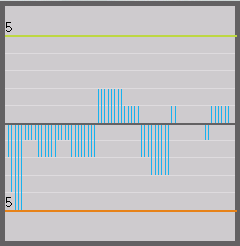
\includegraphics[width=1.25in]{./images/cont1/Viz_6_1}}
		\caption{\textbf{Graph1.} A chart showing change in balance over time. }\label{fig:graph1}
	\end{subfigure}
\quad
	\begin{subfigure}[t]{1.25in}
		\centering
		\setlength\fboxsep{0pt}
\setlength\fboxrule{0.5pt}
\fbox{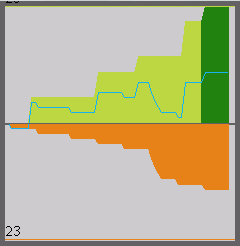
\includegraphics[width=1.25in]{./images/cont1/Viz_8_4}}
		\caption{\textbf{Graph2.} A chart showing change in balance over time, and summed up. }\label{fig:graph2}
	\end{subfigure}


	\caption{Paper prototype visualizations}\label{fig:1}
\end{figure}


\subsection{Results and Discussion}
We rated visualizations based on the number of No. 1 rankings it received.  

In the graph section, we saw that participants strongly preferred Graph2, giving it 10 No. 1 rankings. However, feedback overall was that the graphs were challenging to understand at a glance, and needed more explanation. 

In the visualization section, five participants ranked Viz1 No. 1, making it clearly preferred. Participants liked the ``meter'' and the comparison it provided (P2). It was also remarked to be ``clear, straightforward'', that it ``seems useful'' and ``shows a good balance [of detail]'' (P5).  Viz3 received all No. 4 and No. 5 rankings, because it ``does not show progress and amounts'' (P12), and is ``more confusing'' (P7) . Viz5 received a wider range of rankings, the feedback on it was strong (it is ``a little too judgmental'', and ``not neutral enough'' [P3];P5: ``means nothing with respect to food, smileys are annoying''; P2: ``faces are more discouraging than encouraging-critique''). 
 
Feedback from users indicated that Viz1 is the preferred visualization. Participants liked that it showed the current energy balance and progress toward daily goals or targets, for both energy intake and expenditure. Feedback indicates that the most simple feedback shown (direction and magnitude of energy imbalance, Viz3) does not show enough information and is unsatisfying. Generally, participants found the time-based visualizations too complicated to quickly understand. They also did not believe that the depiction of energy balance over time was useful information. 

Feedback also indicated that participants felt the physical metaphors, such as the scales depicted in Viz4 and Viz5, were too symbolically rich. The imagery was too evocative for simple feedback. The scale metaphor reminded users that if their energy balance was off, their own scale would be tipping. 

Participants did not like the use of money to represent caloric intake and expenditure. While the money ``earned versus spent'' metaphor could be powerful to communicate the ``calories in equals calories out'' concept, people reported that both money and weight were too emotionally charged and they did not want to put the two together. The smiley faces in Viz5, while encouraging when the user is meeting their target, can be discouraging when the user is struggling. Indeed, this is consistent with \cite{consolvo_flowers_2008}, which explores communicating positive and negative affect in feedback mechanisms. 

\section{Prototype, V1 (Feature Phone \& USDA Food Database)}
The next phase of the BALANCE project was the design and development of the first mobile phone prototype. Three things informed the design of this prototype: a review of existing related products (to identify key desired features); a paper prototype process; and the visualization feedback process described above. 

This prototype was built on the Symbian S60 feature phone platform (a top-of-the-line mobile phone platform at the time). Characteristics of mobile phones running the Symbian S60 platform included a relatively powerful processor and ample storage, the ability to develop and run custom software, and high quality cameras. However, they had small displays and 12-key keypads. 

This prototype used the common, freely available USDA Standard Reference. food database (SR19) \citep{u.s._department_of_agriculture_usda_2006}. We added an index based on the FOOD\_DES.FoodName column.  



\begin{figure}	
	\centering
	\begin{subfigure}[t]{1.25in}
		\centering
		\setlength\fboxsep{0pt}
\setlength\fboxrule{0.5pt}
\fbox{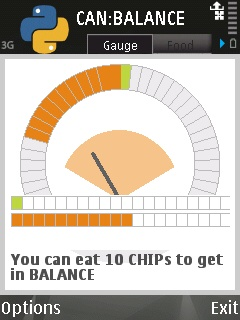
\includegraphics[width=1.25in]{./images/cont1/fig3a}}
		\caption{The home screen depicting overall balance.}\label{fig:fig3a}
	\end{subfigure}
\quad
\begin{subfigure}[t]{1.25in}
		\centering
		\setlength\fboxsep{0pt}
\setlength\fboxrule{0.5pt}
\fbox{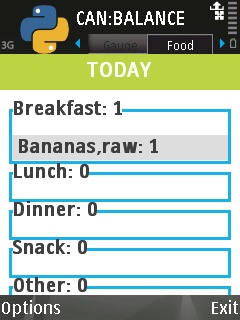
\includegraphics[width=1.25in]{./images/cont1/fig3b}}
		\caption{The food diary, to enter energy intake.}\label{fig:fig3b}
	\end{subfigure}
\quad
\begin{subfigure}[t]{1.25in}
		\centering
		\setlength\fboxsep{0pt}
\setlength\fboxrule{0.5pt}
\fbox{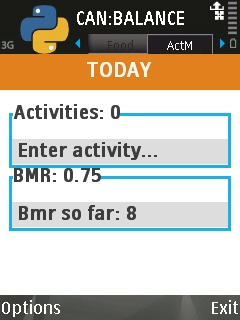
\includegraphics[width=1.25in]{./images/cont1/fig3c}}
		\caption{The activity diary, or energy expenditure.}\label{fig:fig3c}
	\end{subfigure}
\quad
\begin{subfigure}[t]{1.25in}
		\centering
		\setlength\fboxsep{0pt}
\setlength\fboxrule{0.5pt}
\fbox{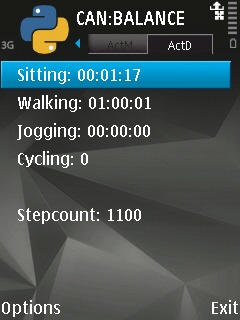
\includegraphics[width=1.25in]{./images/cont1/fig3d}}
		\caption{Sensed activity data from the MSB.}\label{fig:fig3d}
	\end{subfigure}

	\caption{Nokia prototype main screens. }\label{fig:nokiaMainScreens}
\end{figure}


\subsection{Description}
The BALANCE software consisted of four main screens (see Figure \ref{fig:nokiaMainScreens}): The overall balance visualization (Figure \ref{fig:fig3a}), the food diary that shows which foods have been entered today (\ref{fig:fig3b}), and two activity screens. The first activity screen (\ref{fig:fig3c}) shows both intentional activity not detected by the MSB (e.g., water sports such as swimming) and energy expenditure due to base metabolic rate. Base metabolic rate (BMR) is the number of calories a body uses for basic metabolic processes such as breathing. The second activity screen (Figure \ref{fig:fig3d}) shows activity detected by the MSB unit and its contribution to overall energy expenditure. 

\begin{figure}	
	\centering
	\begin{subfigure}[t]{1.25in}
		\centering
		\setlength\fboxsep{0pt}
\setlength\fboxrule{0.5pt}
\fbox{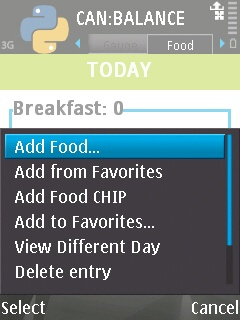
\includegraphics[width=1.25in]{./images/cont1/fig4a}}
		\caption{Select `Add Food' menu item.}\label{fig:fig4a}
	\end{subfigure}
\quad
\begin{subfigure}[t]{1.25in}
		\centering
		\setlength\fboxsep{0pt}
\setlength\fboxrule{0.5pt}
\fbox{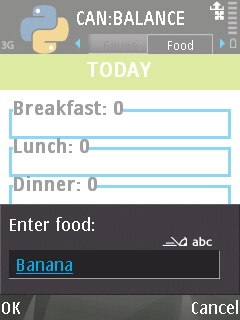
\includegraphics[width=1.25in]{./images/cont1/fig4b}}
		\caption{Enter the name of the food eaten. }\label{fig:fig4b}
	\end{subfigure}
\quad
\begin{subfigure}[t]{1.25in}
		\centering
		\setlength\fboxsep{0pt}
\setlength\fboxrule{0.5pt}
\fbox{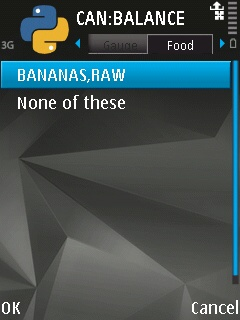
\includegraphics[width=1.25in]{./images/cont1/fig4c}}
		\caption{The software first displays previously used entries with the given name.}\label{fig:fig4c}
	\end{subfigure}
\quad
\begin{subfigure}[t]{1.25in}
		\centering
		\setlength\fboxsep{0pt}
\setlength\fboxrule{0.5pt}
\fbox{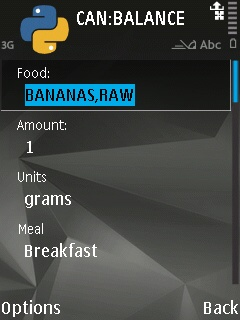
\includegraphics[width=1.25in]{./images/cont1/fig4d}}
		\caption{Selecting the desired food shows this screen, where details about the food entry can be specified. }\label{fig:fig4d}
	\end{subfigure}
\quad
\begin{subfigure}[t]{1.25in}
		\centering
		\setlength\fboxsep{0pt}
\setlength\fboxrule{0.5pt}
\fbox{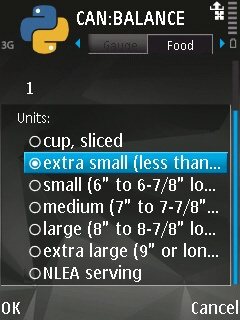
\includegraphics[width=1.25in]{./images/cont1/fig4e}}
		\caption{Selecting the serving amount unit. Some serving units are very specific and natural. }\label{fig:fig4e}
	\end{subfigure}
\quad
\begin{subfigure}[t]{1.25in}
		\centering
		\setlength\fboxsep{0pt}
\setlength\fboxrule{0.5pt}
\fbox{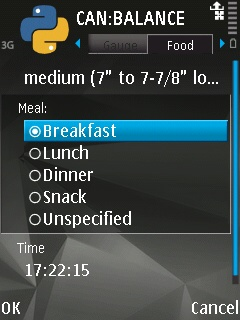
\includegraphics[width=1.25in]{./images/cont1/fig4f}}
		\caption{Selecting the meal for this food.}\label{fig:fig4f}
	\end{subfigure}
	\caption{Nokia prototype: Add known food}\label{fig:fig4}
\end{figure}

In Figure \ref{fig:fig4}, the screenshots depict the process of adding \textit{Banana} to today's food diary. The user first selects ``Add Food'' from the menu. He then types in the term using T9 or multitap. On submit, a list of foods that the user has entered before is shown. The user selects \textit{Banana, Raw}, and is shown a screen to modify the amount, time, and meal eaten. The USDA database provides default serving sizes in grams. Some entries have alternate serving sizes available. For \textit{Banana, Raw}, the serving sizes include ``cup, sliced'' and ``small (6'' to 6 7/8'' long). Finally, the food entry is created. When the food entry is created, the food name appears on the food diary screen and the main visualization is updated. 

\begin{figure}	
	\centering
	\begin{subfigure}[t]{1.25in}
		\centering
		\setlength\fboxsep{0pt}
\setlength\fboxrule{0.5pt}
\fbox{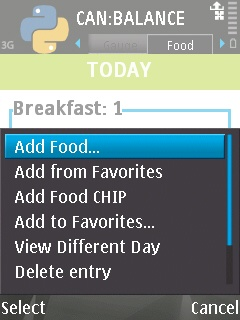
\includegraphics[width=1.25in]{./images/cont1/fig5a}}
		\caption{To make a new food entry, select the `Add Food' menu item. }\label{fig:fig5a}
	\end{subfigure}
\quad
\begin{subfigure}[t]{1.25in}
		\centering
		\setlength\fboxsep{0pt}
\setlength\fboxrule{0.5pt}
\fbox{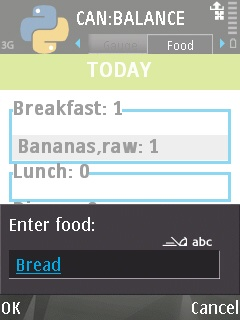
\includegraphics[width=1.25in]{./images/cont1/fig5b}}
		\caption{Enter the food name. }\label{fig:fig5b}
	\end{subfigure}
\quad
\begin{subfigure}[t]{1.25in}
		\centering
		\setlength\fboxsep{0pt}
\setlength\fboxrule{0.5pt}
\fbox{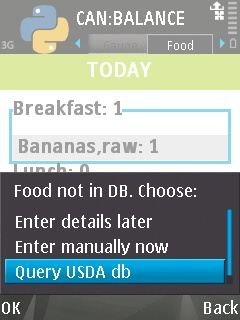
\includegraphics[width=1.25in]{./images/cont1/fig5c}}
		\caption{When the food name has not been used before, the user is given the option to either bookmark the entry to fill out later, create a manual entry using the nutrition facts label now, or query the database.}\label{fig:fig5c}
	\end{subfigure}
\quad
\begin{subfigure}[t]{1.25in}
		\centering
		\setlength\fboxsep{0pt}
\setlength\fboxrule{0.5pt}
\fbox{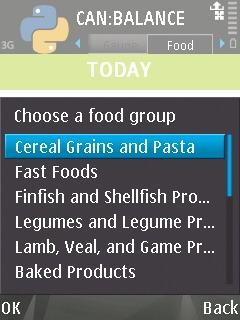
\includegraphics[width=1.25in]{./images/cont1/fig5d}}
		\caption{When there are many entries, the user is asked to choose a food group to filter the results. }\label{fig:fig5d}
	\end{subfigure}
\quad
\begin{subfigure}[t]{1.25in}
		\centering
		\setlength\fboxsep{0pt}
\setlength\fboxrule{0.5pt}
\fbox{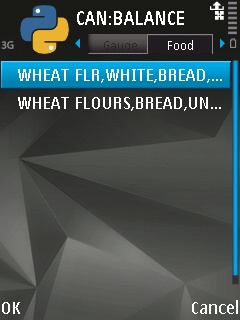
\includegraphics[width=1.25in]{./images/cont1/fig5e}}
		\caption{All matching entries are displayed alphabetically. }\label{fig:fig5e}
	\end{subfigure}
\quad
\begin{subfigure}[t]{1.25in}
		\centering
		\setlength\fboxsep{0pt}
\setlength\fboxrule{0.5pt}
\fbox{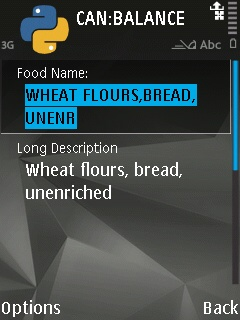
\includegraphics[width=1.25in]{./images/cont1/fig5f}}
		\caption{The user is given a chance to edit the food name to something more recognizable if desired. }\label{fig:fig5f}
	\end{subfigure}
	\caption{Nokia prototype: Adding newly encountered (previously unused) food}\label{fig:fig5}
\end{figure}

One primary goal of this project was for users to be able to quickly and accurately enter exactly how many calories they had consumed. This required finding the most appropriate, exact food and entering it in the exact amount, right after eating. The process of finding food needed to be fast to minimize interruption to the user. Queries to the entire food database took a long time to execute (this is described in further detail later), so to improve performance we separated the database into two separate databases: the entire USDA database and foods the user has entered before. The second database is called the \textit{personal database}. We justify the use of the personal database because many people have a relatively small number of foods they eat on a regular basis (\citep{jastran_eating_2009}). The smaller personal database can be populated over time.  The personal database reduces the amount of time it takes to find a food because it contains fewer foods than the USDA database. This results in a lower query response time. It is also more likely to return the desired food, because it is populated with foods the user has eaten before. 

When the user submits a search, the app first checks the personal database. This first check is fast because the personal database is small. If there are no results, the user is asked whether they want to ``enter later'', ``enter manually'', or ``look up in USDA db''. The ``enter later'' option is essentially a bookmark. This provides a quick alternative to finding the food in the USDA database, which is time-consuming. The ``enter manually'' option provides a form for the user to make an entry based on the Nutrition Information panel required to be printed on all packaged foods. 

Figure \ref{fig:fig5} shows the process of entering a food (\textit{bread}) that has not been entered in the food diary before; therefore, it does not exist in the personal database. When the user query \textit{bread} is not found in the database, the user is given the option to look it up in the USDA database (Figure \ref{fig:fig4c}). If this option is selected and the query returns with foods that belong in more than one food class, the food classes are listed first. Choosing a food class filters the food results list. In this example, the search for \textit{bread} resulted in foods in 14 food classes, which is displayed in three pages of choices (Figure \ref{fig:fig4d}). Choosing \textit{Cereal Grains and Pasta} displays the relevant food results (Figure \ref{fig:fig4e}). The users chooses the item they ate and can modify the name or details. The new food is added to the personal database so that the next time the user enters that food, it can be found faster. Finally, the user specifies the details needed to add the item to the food diary. 

\subsection{Database Optimization and Querying}
One challenge of working with databases is identifying queries the user will make, or want to make, and the expected results. Then, we generate a database query to provide the results. Generating a query based on user input has performance implications, particularly when working with text. Queries on a string column are slower than other data types. Searching for strings with wildcards further degrades the response time. 

In the BALANCE software, a user provides a basic query and the software generates a query based on that user input. Each word the user provides becomes a predicate in the query. This approach results in queries that are known to have poor performance, but this is necessary to account for the ordering of relevant terms in the database. Table \ref{tab:table1} gives some examples of food terms that a user might enter and some example results. As we see in the example of \textit{cream cheese}, if the query had been restricted to ``LIKE �*cream cheese*�'', ``cheese, cream'' would not be returned as a result. There is no simple, systematic way to consistently reorder queries the user provides to match the inconsistent entries in the database. 
 
% Table generated by Excel2LaTeX from sheet 'Sheet1'
\begin{table}[htbp]
\small
  \centering
  \caption[Examples of a user query and results.]{Examples of a user's initial query, how it gets converted into a database query, and some example results. Note that some queries can generate many different, potentially unexpected results. The generated query and subsequent results do not preserve the user's original word ordering. }
    \begin{tabular}{p{1.5in}p{2.2in}p{1.75in}}

    \toprule
%\vtop{\vskip -\ht\strutbox }
    \textbf{User Search Request} & \textbf{Query WHERE clause} & \textbf{Example results} \\
    \midrule
    \textit{cheese} & LIKE �*cheese*�  & Cheese, Cheddar \newline
Cheese, Cream \newline
Bagel with Cream Cheese \newline
Pizza, Cheese and Pepperoni \\
& & \\
   \textit{cream cheese} & LIKE �*cream*� AND LIKE �*cheese*� & Cheese, Cream \newline 
Bagel with Cream Cheese \\
    \bottomrule
    \end{tabular}%
  \label{tab:table1}%
\end{table}%


\subsection{Observations}
Evaluating the first prototype of the BALANCE software revealed many unanticipated difficulties. In this section, I describe the observed problems. They generally relate to the process of finding and choosing a food for the food diary. A summary list is shown below, and I further describe each difficulty: 
\begin{enumerate*}
\item Text entry was difficult. 
\item Querying the database was slow. 
\item Finding and choosing a specific food. 
\begin{itemize*}
\item Using food class to filter search results. 
\item Long names that did not fit on the screen. 
\item No entry for commonly prepared foods. 
\item For some foods, many variations to choose from. 
\end{itemize*}

\end{enumerate*}

\subsubsection{Text entry was too hard}
The 12-key keypad required users to use multi-tap or T9 to enter the names of food they have eaten. This is very difficult to do for foods with long names. When users wanted to enter a food, they needed to decide whether to type in a long, detailed food name, or a short, broad food name. The long and detailed name will likely return fewer food results, but there is a greater chance that the target food is missed. Using a short food name for a query could result in many responses to navigate. 

\textbf {Recommendation: } To appeal to less tech-savvy consumers, provide a more comfortable means of text input. 

\subsubsection{Too long to search}
As discussed above, user input is converted into a query that is known to have poor performance. This is partly due to a mismatch between what the user wants to search for (\textit{cream cheese}) and how it may be stored in the database (``cheese, cream'' or ``bagel, with cream cheese''). It is important that the software returns all of the results. 

The long search time is primarily due to the limited resources on the mobile phone. The database available on the mobile platform has reduced capabilities as compared to those available on a desktop or in a high performance computing environment. The limited processing power of the device magnifies the limitations of the database. 

\textbf {Recommendation:} Faster hardware, improve the filtering process.
 
\subsubsection{It was difficult to find and choose a food}
After entering a food query and waiting for the search to return, a user needs to choose the desired food from all of the results. 
Using food class to filter search results. As noted earlier, if the results are from just one food class, the entire list of results is immediately shown. If there are results in multiple food classes, the list of food classes is shown to allow the user to choose the most appropriate. To find the target food, the user must choose from a potentially long list of food classes (the results for the query \textit{bread} include 16 food classes). Some of the food classes are difficult to distinguish. For example, the food classes for \textit{Bread} includes both ``Cereal Grains and Pasta'' and ``Baked Goods''. This requires the user to make a decision, and users unfamiliar with the food classes are not sure which to choose. 

\textbf{Recommendation: }Do not force the user to think about arbitrary food classes. Provide guidance about what each food class represents. Provide some ``teasers'' or a few items of that food class to demonstrate what kinds of foods it contains. 

\subsubsection{Long names do not fit on the screen.}
The USDA database contains food descriptions that are long and descriptive. For example, a typical entry for the query ``Steak'' is ``Beef, short loin, porterhouse steak, separable lean and fat, trimmed to 1/4'' fat, USDA choice, raw''.  The alternative ``short'' description is a similar entry using defined abbreviations: ``Beef, shrt loin,prtrhs steak,ln,1/4'' fat,usda choic,raw''. Neither of these descriptions display well on the small screen size of the target device. If they are displayed one entry per line in a font that is comfortable to read, not enough words are shown to distinguish one entry from another. If the description is shown on multiple lines, only one or two entries can be shown at a time. Forcing the user to select one to see more detail and then returning to the list screen is time consuming and frustrating. 
 
\begin{figure}[ t ]
\begin{center}

\setlength\fboxsep{0pt}
\setlength\fboxrule{0.5pt}
\fbox{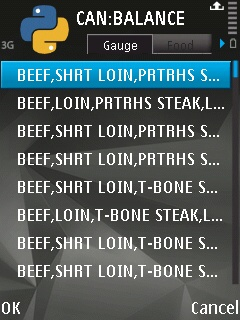
\includegraphics [ width=1.25in ]{./images/cont1/fig6}}

\caption{Nokia prototype: `Steak' results}
\label{fig:fig6}
\end{center}
\end{figure}

\textbf {Recommendation: }Use a larger display with higher resolution. Use a database that has more useful short descriptions. Structure the database to provide a short ``food name'', a short description, and a detailed description. 

\subsubsection{No entries for common prepared foods. }
The USDA database is that it did not include many prepared foods, such as those purchased at a grocery store or restaurant. The database contains food entries from only 60 manufacturers. This includes some of the major food manufacturers in the US (e.g. Burger King, Kellogg, Nestle, McDonalds). However, users expect that if they can purchase a food (e.g., it has a UPC code), then it will be in the database. 

\textbf{ Recommendation:} Choose a database that includes a more comprehensive list of prepared foods. 

\subsubsection{For some foods, many items to choose from.}  For some foods, there are many entries that appear very similar. For example, a query for \textit{cheese} in the ``Dairy and Egg Products'' Food Class has 44 entries. The cheese entries include: cheese, blue; cheese, brick; cheese, brie;  cheese, camembert; cheese, cheddar; etc. Some results may be unfamiliar to a user, but the text of each result is noticeably different from the others. The results for \textit{Porterhouse} (steak) are not so clearly different. The list below displays the full name of six results for \textit{porterhouse}: 

\begin{itemize*}
\item Beef, short loin, porterhouse steak, separable lean and fat, trimmed to 0'' fat, all grades, cooked, broiled
\item Beef, short loin, porterhouse steak, separable lean and fat, trimmed to 0'' fat, USDA choice, cooked, broiled
\item Beef, short loin, porterhouse steak, separable lean and fat, trimmed to 0'' fat, USDA select, cooked, broiled
\item Beef, short loin, porterhouse steak, separable lean only, trimmed to 0'' fat,  all grades, cooked, broiled
\item Beef, short loin, porterhouse steak, separable lean only, trimmed to 0'' fat, USDA choice, cooked, broiled
\item Beef, short loin, porterhouse steak, separable lean only, trimmed to 0'' fat, USDA select, cooked, broiled
\end{itemize*}

The six results vary on two factors: whether the item contains only the separable lean meat, or the meat and fat; and the grade rating of the meat, USDA choice, select, or any. 

This amount of detail confuses users. They report uncertainty about which one most accurately reflects the food they ate, and question whether the difference between all these results is significant. Additionally, the amount of distinguishing detail for this entry makes users wonder if they should be capturing that amount of detail for all of the foods they enter. This compounds the previous problem of not being able to find prepared foods: given the level of detail required to document a piece of steak, how should the user document a piece of pizza, which vary wildly due to toppings and preparation?

\textbf{Recommendation:} Use a database that was designed for use by a consumer rather than an expert. 

The overall process to add food to the food diary is too long, due to all of the factors described in detail above. For the BALANCE project, it was important that users are able to enter foods quickly, so that they are able to enter food throughout the day and ensure the fuel-gauge visualization is properly updated. 

\subsection{Discussion}
The Nokia-USDA BALANCE prototype exposed some inherent challenges of designing and developing a food diary for a mobile phone. The challenges are due partly to the database, and partly from using a device with limited interaction modes to navigate a challenging data environment. Our target population is a general population, not necessarily very comfortable entering text via multitap or T9. This challenge of text entry magnifies the problem of querying the database and navigating the results. 

One conclusion from this process was to use a different mobile phone. The original Symbian S60 device was much friendlier to use and more powerful than previous smartphones, but the target population had little smartphone experience.  Text entry was one of the biggest barriers: the 12-key keypad with multitap or T9 input was not comfortable to most consumers. 

The database negatively impacted the navigation and performance. Database entries were not well suited to the mobile phone display, and the query process on the device was too slow. It is also necessary to have more popularly available packaged or prepared foods, although some of the closely related foods could be collapsed. The importance of the database in self-monitoring or dietary assessment is outlined in \cite{stumbo_considerations_2008}. Indeed, they state ``Mastery of computerized dietary assessment requires an understanding of the database in terms of the naming conventions, the search strategy for finding foods, and data completeness for generic and brand-name foods.'' This is consistent with our experiences. 

\section{Food Databases}
Food diaries have conflicting requirements for the food database. In particular for BALANCE, the database needs to be quick to search (small), yet have the foods that people eat and are looking for (large). It also needs to be able to distinguish between similar items, and use terminology that is familiar to the target user population. Grouping into friendly and familiar food groups or classes will help users to find food in the database by providing data to filter on or browse. Providing useful, appropriate serving sizes is another helpful feature. For example, the food entries for \textit{Coca Cola} should have commonly available serving sizes to choose from, such as a 12-oz can, a 20-oz bottle, or a 16-oz cup, even though the USDA-defined `typical' serving size for soda is 8 oz. 

The characteristics of food databases can be better appreciated within the historical context. Generally, food databases are used by professionals who are experts in food service, preparation, and evaluation. Hospitals, nursing homes, and other medical facilities use food databases to ensure patients are fed properly, fulfilling individual requirements. They generate menus for days, weeks and months, using the database to ensure proper nutrition for all recipients over time. Nutritionists and registered dietitians use commercial food databases to work with clients who have certain dietary constraints--- either to look up foods that an individual ate and evaluate their diet overall, or to generate a meal plan for an individual and provide detailed information about it. Organizations such as daycares, schools and prisons (particularly if they are government funded) use food databases to ensure that they meet governmental guidelines. Food manufacturers use food databases to generate Nutrition Facts labels for their products. 

For the tasks outlined above, the end user of the database is an expert who is familiar with food systems, organization, and terminology. The user has formal training and uses the database on a regular basis. However, increasingly, food databases have been made available to the general population, usually in the form of a consumer tool to support weight loss. 

Table \ref{tab:foodDbCompare} provides some information on two databases: the USDA (SR21) database we used for the first prototype, and the NPKB that we used for the next version of the software. In addition to containing information for many more foods, it also provides more food serving sizes that could make it easier for users to specify how much they have eaten. It also contains foods from many more manufacturers, which can help address the expectation to find processed or prepared foods in a database. Finally, the NPKB database contains more foods groups, organized in a hierarchical fashion. The large number of food groups and hierarchy may help users find a food they are looking for. 

% Table generated by Excel2LaTeX from sheet 'Sheet2'
\begin{table}[htbp]
\small
  \centering
\begin{minipage}{\textwidth}
\centering

    \begin{tabular}{p{2in}p{1.75in}p{1.75in}}
    \toprule
    \textbf{} & \textbf{USDA} & \textbf{Nutritionist Pro Knowledge Base} \\
    \midrule
    \textbf{Version} & SR21 (Sept 2008) & V44 (Fall, 2009) \\
    \textbf{File size\footnote{Access database file size}} & 16.5 Mb & 135 Mb \\
    \textbf{Number of foods} & 7,412 & 39,194 \\
    \textbf{Number of food servings\footnote{``serving types''}} & 13,087\footnote{Number of records in the `Weight' table.}  & 46,722\footnote{Number of records in the `tblFoodServingTypes' table} \\
    \textbf{Number of serving types} & 1,700  & 5,087 \\
    \textbf{Number of manufacturers} & 60    & 592 \\
    \textbf{Number of recipes} &       & 783 \\
    \textbf{Food groups} & 24    & 369\footnote{Food Classes. Includes all hierarchy.}\\
    \textbf{Number of nutrients } & 140   & 90 \\
	\bottomrule~
    \end{tabular}%
\end{minipage}
  \caption{Comparing nutrition databases\label{tab:foodDbCompare}}  
	%
\end{table}%




 
\section{Food Diary: Iterative Design And Evaluation}
In this section, I describe the design and features of the food diary portion of the overall BALANCE project. The challenges identified in the previous section informed the decision to move to a Windows Mobile platform and adopt a commercially available nutrition database to drive the food diary. The combination of the paper prototype user study and Symbian implementation informed the new design on the Windows Mobile platform. The final design was informed by an iterative, user-centered evaluation process. 

Focus groups of 4-5 participants provided user feedback in the design and development process. We convened five focus groups over a seven month period. We provided participants a mobile phone running the food diary software. We asked to track what they eat for three days prior to the focus group. After the three days of tracking and before the focus group, participants completes two usability questionnaires (CSUQ and MPUQ, \citep{lewis_ibm_1995, ryu_reliability_2006}). The focus group was moderated by a team member. Topics focused on what the participants liked, what worked and did not work, and features they would like to see added. Details are in \citet{hughes_balance_2010}. Feedback from the participants in the focus groups provided input to the design and development of the next software iteration. 
We used two metrics to evaluate the overall progress of the iterative process. First, we analyzed usability questionnaire responses over time. These did not show a significant improvement of the usability of the food diary software overall. The other measure of progress we considered was the time between when a participant ate a food and when they entered it in the food diary. We hypothesized that this time would decrease as the food diary improved. This also did not show a significant improvement of the food diary. Details of the analysis are provided in \citet{hughes_balance_2010}. I also discuss the use of these metrics later in this section and in Chapter \ref{cha:cont4}. 

\subsection{Overall Design}
The final version of the BALANCE software ran on a Windows Mobile 6.1 Professional device. We chose this device because it had a large display, a touch screen, and a slide-out QWERTY keyboard. Text input can be done either via the physical QWERTY keyboard or with the ``soft input panel'', on-screen keyboard. We used the NutritionistPro Knowledge Base (NPKB) for the food diary. 

\subsubsection{Food Diary Software}
The primary task for the food diary is to enable users to find a food that has been eaten from a database, specify how much of it they ate, and save a record of it. 

\begin{figure}	
	\centering
	\begin{subfigure}[t]{1.25in}
		\centering
		\setlength\fboxsep{0pt}
\setlength\fboxrule{0.5pt}
\fbox{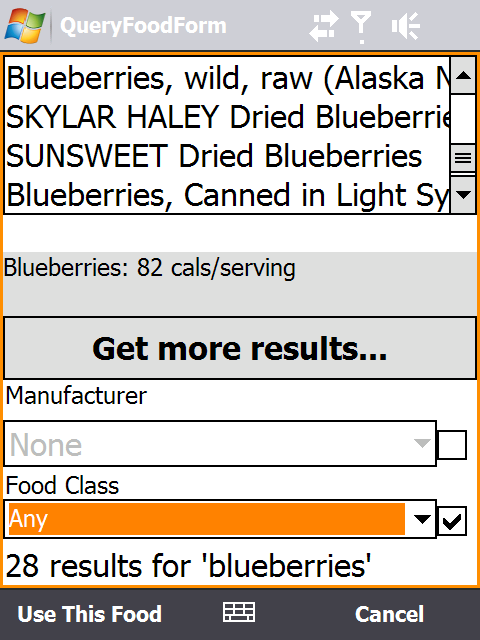
\includegraphics[width=1.25in]{./images/cont1/fig7a}}
		\caption{The BALANCE food diary main screen.}\label{fig:fig7a}
	\end{subfigure}
\quad
\begin{subfigure}[t]{1.75in}
		\centering
		\setlength\fboxsep{0pt}
\setlength\fboxrule{0.5pt}
\fbox{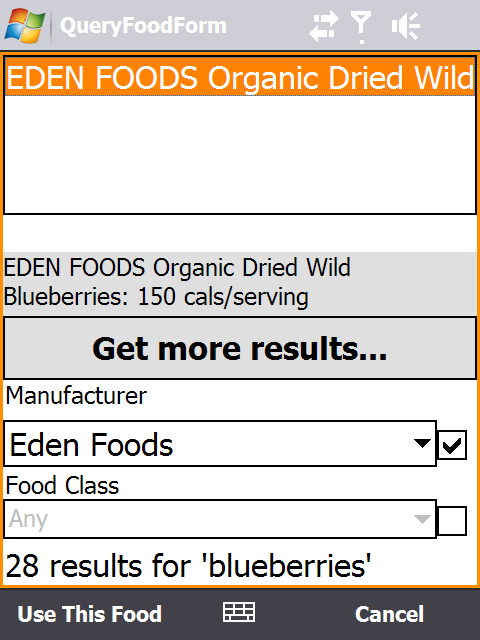
\includegraphics[width=1.75in]{./images/cont1/fig7b}}
		\caption{Entering the query term. Common or previously used results appear.}\label{fig:fig7b}
	\end{subfigure}
\quad
\begin{subfigure}[t]{1.75in}
		\centering
		\setlength\fboxsep{0pt}
\setlength\fboxrule{0.5pt}
\fbox{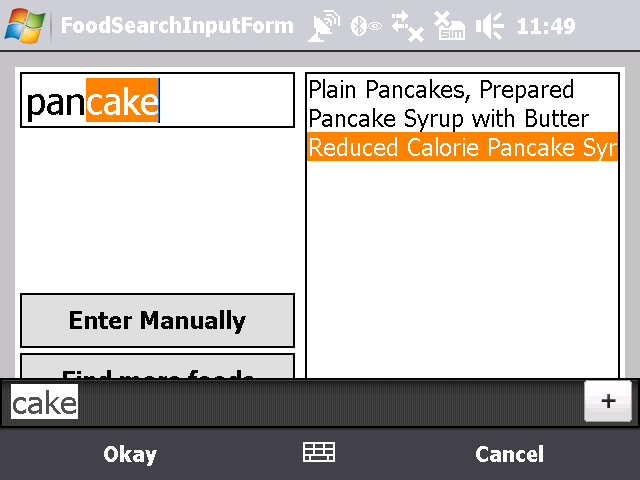
\includegraphics[width=1.75in]{./images/cont1/fig7c}}
		\caption{The user continues typing to filter out this list. }\label{fig:fig7c}
	\end{subfigure}
\quad
\begin{subfigure}[t]{1.25in}
		\centering
		\setlength\fboxsep{0pt}
\setlength\fboxrule{0.5pt}
\fbox{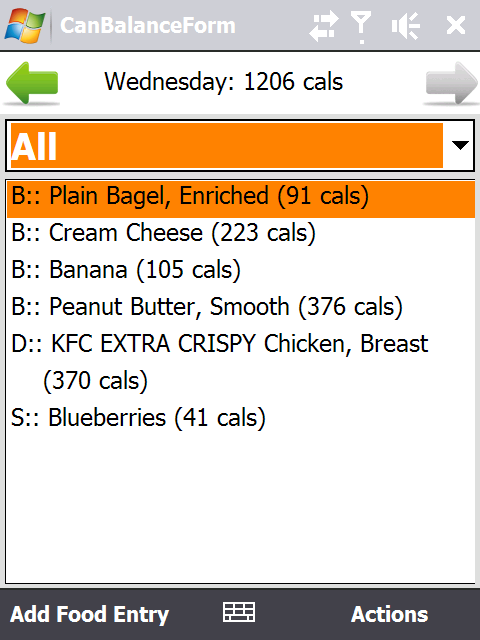
\includegraphics[width=1.25in]{./images/cont1/fig7d}}
		\caption{An exact match was not found, so more results were loaded. This list can be filtered by manufacturer or food class.}\label{fig:fig7d}
	\end{subfigure}
\quad
\begin{subfigure}[t]{1.25in}
		\centering
		\setlength\fboxsep{0pt}
\setlength\fboxrule{0.5pt}
\fbox{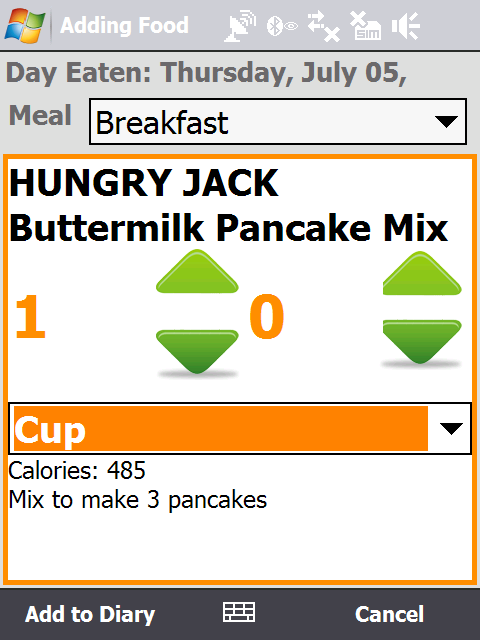
\includegraphics[width=1.25in]{./images/cont1/fig7e}}
		\caption{Creating the entry by specifying the day it was eaten, the meal, and the amount. }\label{fig:fig7e}
	\end{subfigure}
\quad
\begin{subfigure}[t]{1.25in}
		\centering
		\setlength\fboxsep{0pt}
\setlength\fboxrule{0.5pt}
\fbox{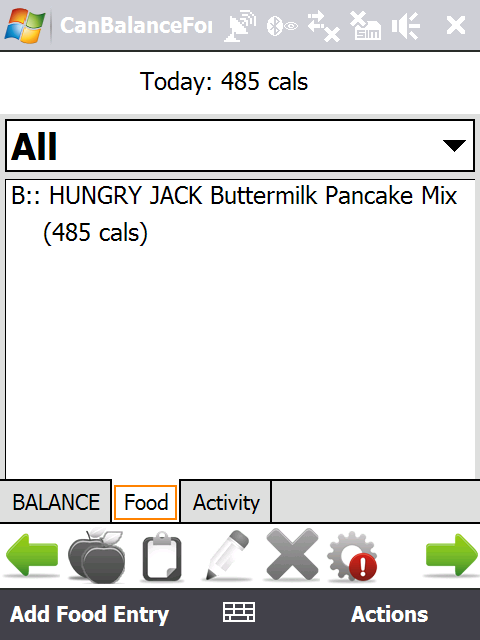
\includegraphics[width=1.25in]{./images/cont1/fig7f}}
		\caption{The new food entry is now displayed on the food diary main screen. }\label{fig:fig7f}
	\end{subfigure}
	\caption{WinMobile food diary.}\label{fig:fig7}
\end{figure}


Figure \ref{fig:fig7} shows the process of adding a food to the diary. The application starts with a list of food that has been eaten today (\ref{fig:fig7a}). The ``Add Food Entry'' button displays a screen that allows the user to start typing an entry (\ref{fig:fig7b}). As the user types, a list of common or recently eaten foods populates the display (\ref{fig:fig7c}). If the user sees what they want, they can either select it, choose to ``Enter Manually'' (create a new entry based on the Nutrition Information label on the package), or ``Find more'', which searches the entire food database (\ref{fig:fig7d}). This list can be filtered by manufacturer and food class  (\ref{fig:fig7d}). Once a food is selected, the user specifies what time they ate the food, which meal it should be counted with, and how much of it they ate  (\ref{fig:fig7e}). The entry is then saved and shown on the daily food list  (\ref{fig:fig7f}). 

\subsection{Selected Features and Feedback}
Throughout the iterative design process, we aimed to improve the existing functionality and add features as necessary. In this section, I detail some of the features that evolved based on user feedback. 

\subsubsection{Touch-friendly screen design }

We chose the final device for its touch-sensitive screen. We believed the touch interface could help reduce the time required to create a food entry, whether the touch was provided by a fingernail or a stylus. Initially, the food diary design supported touch interaction by using traditional WinMobile interface widgets scaled to respond to fingernail touches. This required the widgets to be larger than widgets sized to support stylus interaction (see \ref{fig:fig8}). However, early in the feedback process, users reported that they did not like the stylus. This indicated that they were using it, even though the design did not intend to require it. Although the traditional widgets were scaled to respond to fingernail touches, the appearance invited the use of a stylus for interaction. Additionally, users provided valid complaints against the use of a stylus: it was too small to hold comfortably; users were afraid of losing it; and it was time consuming to take it out and put it back. 

In response to user feedback about the use of the stylus, we redesigned the interface to use custom widgets that invited fingernail touches (see \ref{fig:fig8b} and \ref{fig:fig8c}). Users remarked on the ``friendliness'' and ``cheeriness'' of the new widgets. 

\begin{figure}[tbh]
	\centering
	\begin{subfigure}[t]{1.25in}
		\centering
		\setlength\fboxsep{0pt}
\setlength\fboxrule{0.5pt}
\fbox{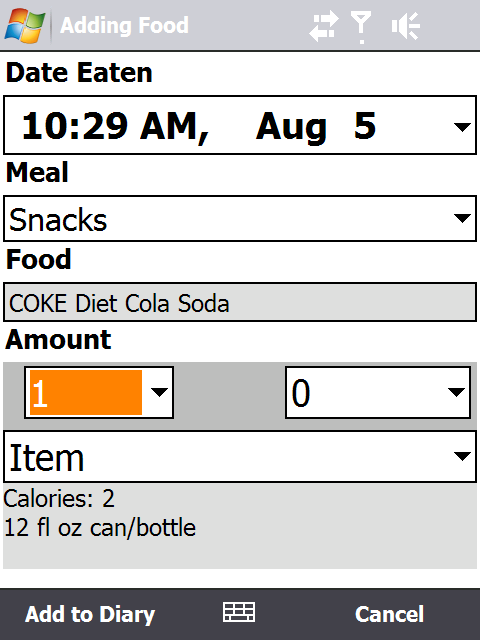
\includegraphics[width=1.25in]{./images/cont1/fig8a}}
		\caption{The first design. The design and layout is typical of a Windows Mobile or PDA software that depends on the use of a stylus. }\label{fig:fig8a}
	\end{subfigure}
\quad
\begin{subfigure}[t]{1.25in}
		\centering
		\setlength\fboxsep{0pt}
\setlength\fboxrule{0.5pt}
\fbox{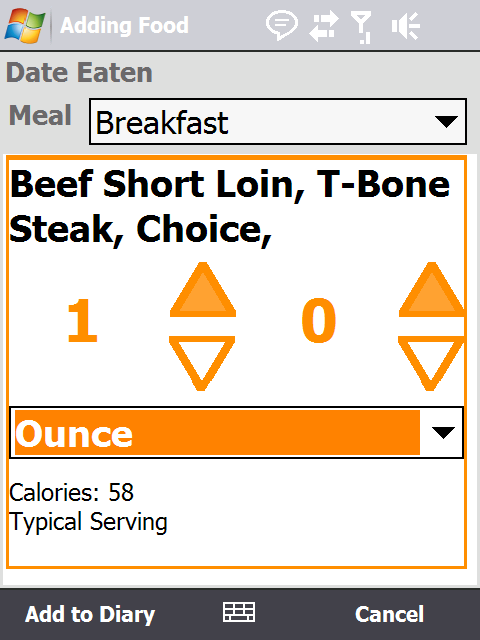
\includegraphics[width=1.25in]{./images/cont1/fig8b}}
		\caption{A revision, with large, finger touch friendly buttons to modify the serving amount.  }\label{fig:fig8b}
	\end{subfigure}
\quad
\begin{subfigure}[t]{1.25in}
		\centering
		\setlength\fboxsep{0pt}
\setlength\fboxrule{0.5pt}
\fbox{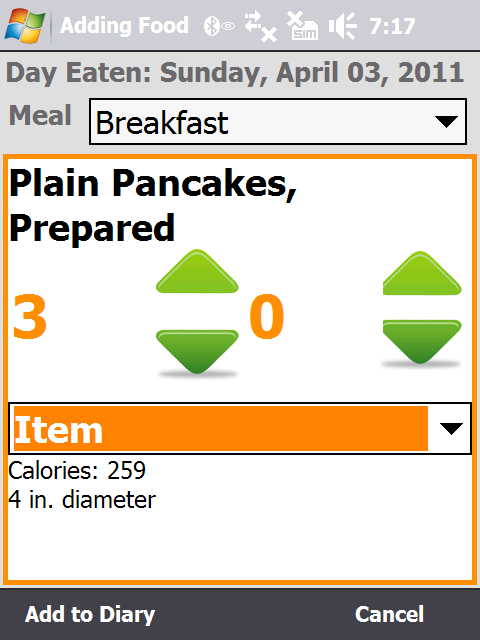
\includegraphics[width=1.25in]{./images/cont1/fig8c}}
		\caption{The final version.}\label{fig:fig8c}
	\end{subfigure}
	\caption{Evolution of serving size specification to make it more touch-friendly.}\label{fig:fig8}
\end{figure}

\subsubsection{Create new food database entry}
The NPKB contained many foods, but users still reported encountering foods that were not in the database. This resulted in the ability to add a new food to the database, using information from the Nutrition Facts label that all packaged foods are required to have. After the entry is created, it shows up in the quick-search results with other common and recently used foods. 
 
\begin{figure}[ t ]
\begin{center}

\setlength\fboxsep{0pt}
\setlength\fboxrule{0.5pt}
\fbox{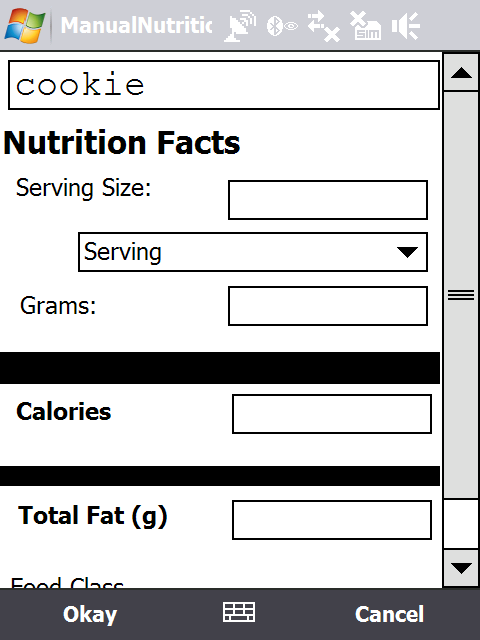
\includegraphics[ width =1.25in ]{./images/cont1/fig9}}
\caption{Add a new manual entry to food diary when the database does not have the desired food. }
\label{fig:fig9}
\end{center}
\end{figure}

\subsubsection{Favorite foods and meals}
Focus group participants repeatedly asked for shortcuts and customization features. In addition to the ability to add a new food to the database described above, participants wanted the ability to bookmark favorite foods and meals. The favorite meals feature is shown in Figure \ref{fig:fig10}. Figure \ref{fig:fig10a} shows the list of all meals that have been marked as a favorite. When the user wants to enter the favorite meal, s/he selects it from the list. Figure \ref{fig:fig10b} shows all of the items in the meal, as well as the amount. The time defaults to the current time (rounded to the nearest 15 minutes). The saved favorite meal includes the meal specification (breakfast, dinner, etc.), which populates the meal widget. The details of the meal can be modified to reflect the current meal (\ref{fig:fig10c}). Finally, when the user confirms, all of the items in the meal are added to the food diary (\ref{fig:fig10d}). 

\begin{figure}	
	\centering
	\begin{subfigure}[t]{1.25in}
		\centering
		\setlength\fboxsep{0pt}
\setlength\fboxrule{0.5pt}
\fbox{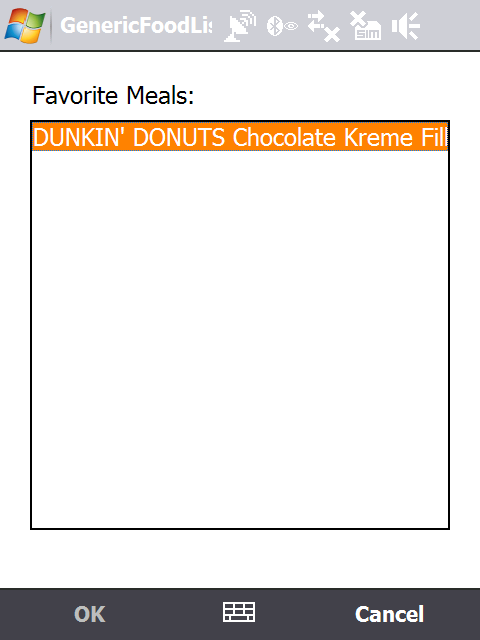
\includegraphics[width=1.25in]{./images/cont1/fig10a}}
		\caption{The list of meals saved as `Favorite'.}\label{fig:fig10a}
	\end{subfigure}
\quad
\begin{subfigure}[t]{1.25in}
		\centering
		\setlength\fboxsep{0pt}
\setlength\fboxrule{0.5pt}
\fbox{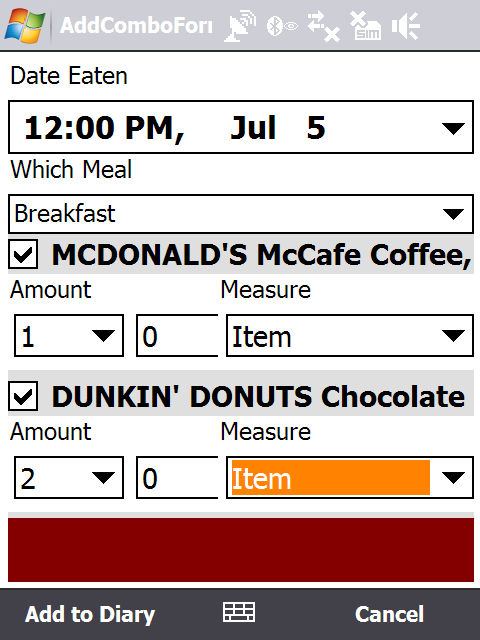
\includegraphics[width=1.25in]{./images/cont1/fig10b}}
		\caption{Selecting a meal shows a screen that lists each item in the meal, including serving sizes. In this case, one McDonald's coffee and two donuts. }\label{fig:fig10b}
	\end{subfigure}
\quad
\begin{subfigure}[t]{1.25in}
		\centering
		\setlength\fboxsep{0pt}
\setlength\fboxrule{0.5pt}
\fbox{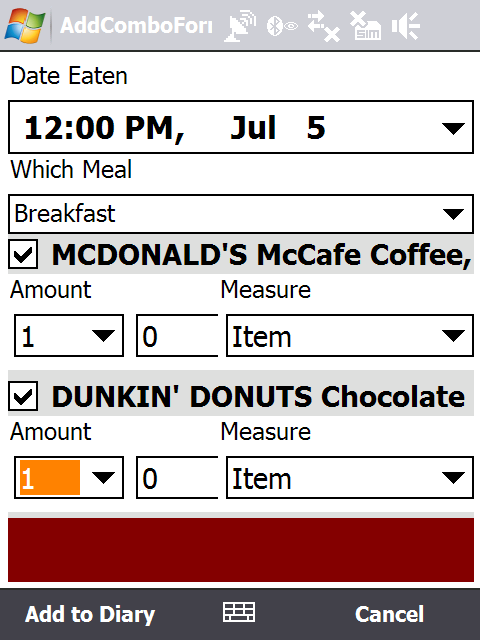
\includegraphics[width=1.25in]{./images/cont1/fig10c}}
		\caption{The amounts can be modified to reflect the current meal. }\label{fig:fig10c}
	\end{subfigure}
\quad
\begin{subfigure}[t]{1.25in}
		\centering
		\setlength\fboxsep{0pt}
\setlength\fboxrule{0.5pt}
\fbox{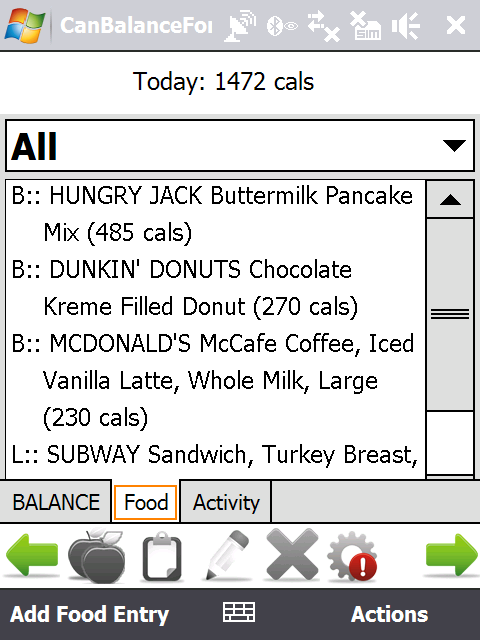
\includegraphics[width=1.25in]{./images/cont1/fig10d}}
		\caption{When entered, each item is added to the daily food list. }\label{fig:fig10d}
	\end{subfigure}

	\caption{Using the favorite meals feature to add entries to the food diary. }\label{fig:fig10}
\end{figure}

\subsection{Database Query Details}
Adopting the commercially available NPKB resulted in a much larger number of foods available to the user. While the USDA database had the user challenge of making it difficult to distinguish between many similar unprocessed foods and relatively few processed/manufactured foods, the NPKB had many more processed and manufactured foods to choose from, which users sometimes found overwhelming. 

In this section, I describe some of the ways we tried to make the query process more user friendly. Rather than describe all the possible improvements we considered, I focus on the final implementation. 

One weakness of the database supported on the Windows Mobile platform (SQL Server CE) is that it does not support full text search. When full text search is available on a database, queries can be made that reflect linguistic characteristics of a given language (such as English). With a FTS capability, one can easily query  not just for a word or a phrase, but a word or a phrase that starts with given text (prefix), inflectional forms of a word (e.g., foot or feet), a word or phrase close to another word or phrase, or a synonymous term. This is valuable in the case of food diaries, because from the user's perspective it is sometimes unclear whether the food diary will have ``Potatoes, Mashed'' or ``Mashed Potatoes'' as an entry. Additionally, consumers in general are familiar with search strategies that employed FTS, whether or not they know enough about it to specify it exactly. Users are able to articulate is that a particular search function ``just knows what I'm looking for'' and ``does the right thing'', linguistically-a search for ``potatoes'' also yields results with ``potato''. 

Full text search also improves the query speeed. The alternative to full text search is a LIKE query based on character patterns. A LIKE query against millions of rows of text data can take minutes to return, while a full text search query can take only seconds (or less) on the same data, depending on the number of rows that are returned. This is due to the pre-built index that full text search generates. 

We attempted to overcome the lack of free-text search on the database by being smart about the queries we generated. However, the more complex a query became, the longer the time to respond, even if the results were ``better''.  In general, our approach favored returning better results faster, rather than minimizing the size of the database. Storage was cheap: we could easily add a larger memory card to the device, but we could not improve the processor. 

To improve the query time and search process, we implemented a lightweight predictive search mechanism. As mentioned above, the system contained two food databases: the large, complete NPKB and a smaller, personalized personal database. The personal database was initially seeded with foods marked as ``common'' or ``generic'' in the NPKB. To improve the responsiveness, there was a table in the personal database that contained the first 3 letters of all words in the food name, description and manufacturer name associated with a food entry. When the user starts typing to search for a food name, after 3 characters are entered, a results box is generated based on an exact string match from that table. As the user continues typing, the list of results is filtered based on that text. If a desired food is not found, the user can ``Find More'', which ends up performing the longer LIKE query on the NPKB. When a food is selected from the NPKB and entered into the food diary, it is also stored in the personal database. The prefix table is then updated. This adds time to the process, but this time is negligible to the time required for the NPKB query. 

\subsection{Metrics}

In this section, I want to talk about the metrics we used to guide the development and evaluation of the software. Specifically, I want to review what we used, how they worked, why they failed, and propose alternate metrics to collect during the final evaluation. 

We defined one measure of software success as the time between when a food was eaten and when it was entered into the diary. This measure did not show  significant improvement, but it did indicate how the software is used. This was supported by feedback in the focus groups. Participants reported that they did not make food entries throughout the day, and were not likely to. Multiple reasons were given for this: sometimes it was just that the person was too busy and could not take the time, and sometimes it was just easier to do it all at once later in the day. Some participants noted that they took advantage of free time, such as waiting for the bus, to review and make food entries. This does not help us to identify if the reluctance to make food entries at the time of eating is due to an inherent tedium in the task, or if the software makes the process more or less challenging. 

This study highlighted the importance of identifying appropriate metrics for evaluating food diaries on cell phones. Good metrics should reflect both usability, or how the software is being used, and domain-- whether users are able to achieve the stated goal (in this case, entering the right number of calories by identifying all eaten foods). 

\section{Validating BALANCE}
The final BALANCE validation combined all key components of the project: the MSB device for calorie expenditure calculation and the mobile phone with the visualization, food diary and activity diary software. Participants were asked to carry the mobile phone and MSB for 4 days. They were asked to enter all food and drink consumed (except water), and manually enter the activity that the MSB did not track. They were asked to record on days 1, 3 and 4, but on the second day they only performed a 24-hr recall of what they ate on the first day. They completed a post-use questionnaire intended to identify useful features, and completed an activity questionnaire. See \citet{snively_balance_2010} for more details. 

\subsection{Final BALANCE Software}
Up until this point, the discussion has focused on the design and development of the food diary and visualization components of the BALANCE project, independently. As mentioned earlier, the entire project consists of the feedback visualization, food diary, activity diary, and activity sensing component (MSB) combined together. In this section, describe the activity portion of the system. 
The activity diary (shown in \ref{fig:fig11c}) shows both activities entered by the user and activity information detected by the MSB. The user is responsible for entering activity not detected by the MSB, such as swimming or vigorous sports. The activity database is based on the Physical Activity Compendium \citep{ainsworth_compendium_2000}. 

\begin{figure}	
	\centering
	\begin{subfigure}[t]{1.25in}
		\centering
		\setlength\fboxsep{0pt}
\setlength\fboxrule{0.5pt}
\fbox{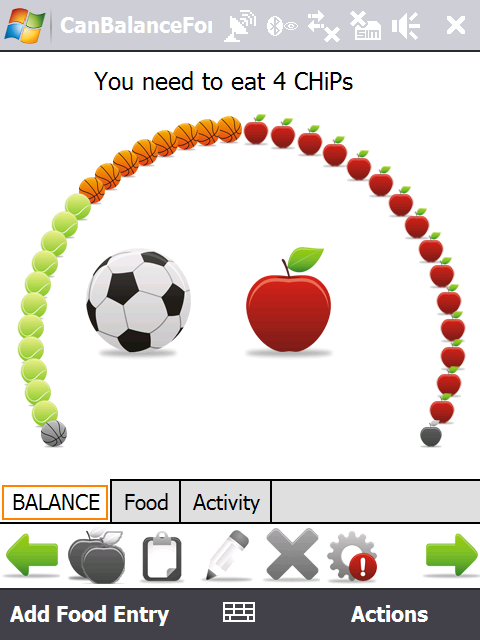
\includegraphics[width=1.25in]{./images/cont1/fig11a}}
		\caption{The home screen with the BALANCE visualization. The orange basketballs indicate CHIPs expended due to BMR. The green tennis balls indicate CHIPs expended due to activity.}\label{fig:fig11a}
	\end{subfigure}
\quad
\begin{subfigure}[t]{1.25in}
		\centering
		\setlength\fboxsep{0pt}
\setlength\fboxrule{0.5pt}
\fbox{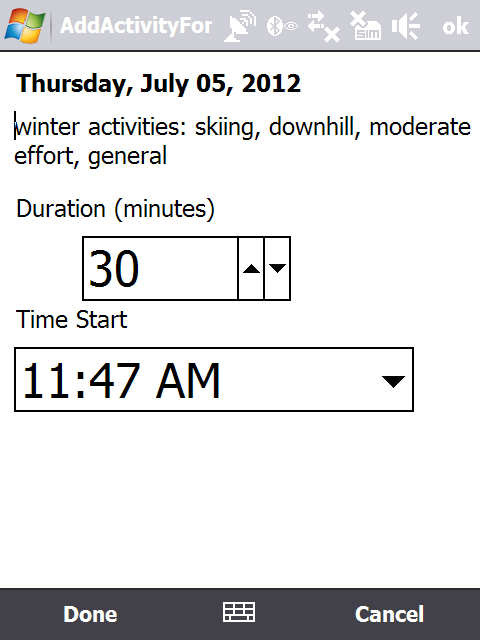
\includegraphics[width=1.25in]{./images/cont1/fig11b}}
		\caption{Adding a physical activity to the diary. The MSB is unable to detect some activities. }\label{fig:fig11b}
	\end{subfigure}
\quad
\begin{subfigure}[t]{1.25in}
		\centering
		\setlength\fboxsep{0pt}
\setlength\fboxrule{0.5pt}
\fbox{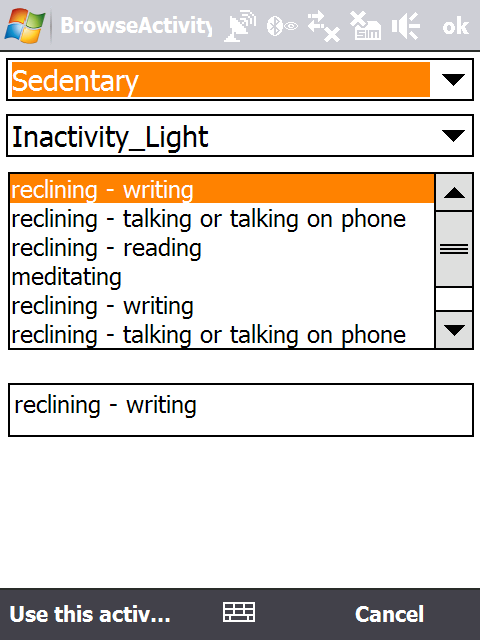
\includegraphics[width=1.25in]{./images/cont1/fig11c}}
		\caption{The list of non-MSB physical activities entered for today.  }\label{fig:fig11c}
	\end{subfigure}
\quad
\begin{subfigure}[t]{1.25in}
		\centering
		\setlength\fboxsep{0pt}
\setlength\fboxrule{0.5pt}
\fbox{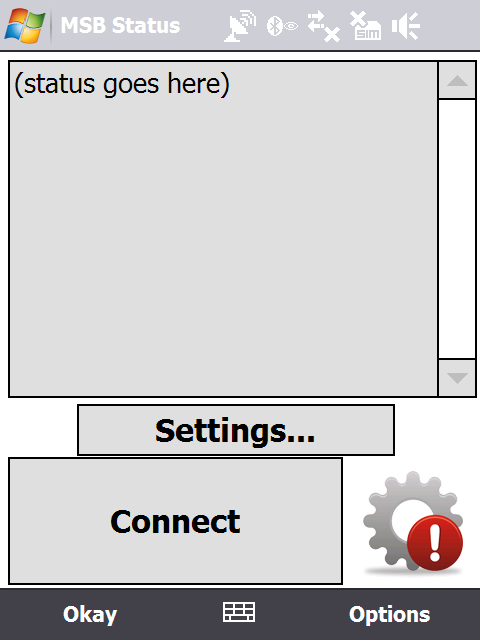
\includegraphics[width=1.25in]{./images/cont1/fig11d}}
		\caption{MSB status and information. }\label{fig:fig11d}
	\end{subfigure}

	\caption{Final BALANCE non-food diary screens.}\label{fig:fig11}
\end{figure}


The pager-sized MSB is worn on the user's hip. It is connected to the phone via a wireless Bluetooth connection. The interface supports connecting to and communicating with the device, displaying information about the sensed activities. The software also monitors the connection and notifies the user if the connection breaks. 


\subsection{24-hr recall software. }
A 24-hr recall is a process in which a trained researcher works with an individual to identify all the foods that the person ate in the past 24 hrs. The protocol is designed to elicit complete and correct dietary intake over the previous 24 hours. The BALANCE validation compared the results from a 24-hr recall to the entries in the mobile phone food diary. This process required a tool for the researcher to access the same food database using the same query process as the BALANCE food diary. We developed a desktop version of the food diary app to support this task. 

\begin{figure}[ t ]
\begin{center}

\setlength\fboxsep{0pt}
\setlength\fboxrule{0.5pt}
\fbox{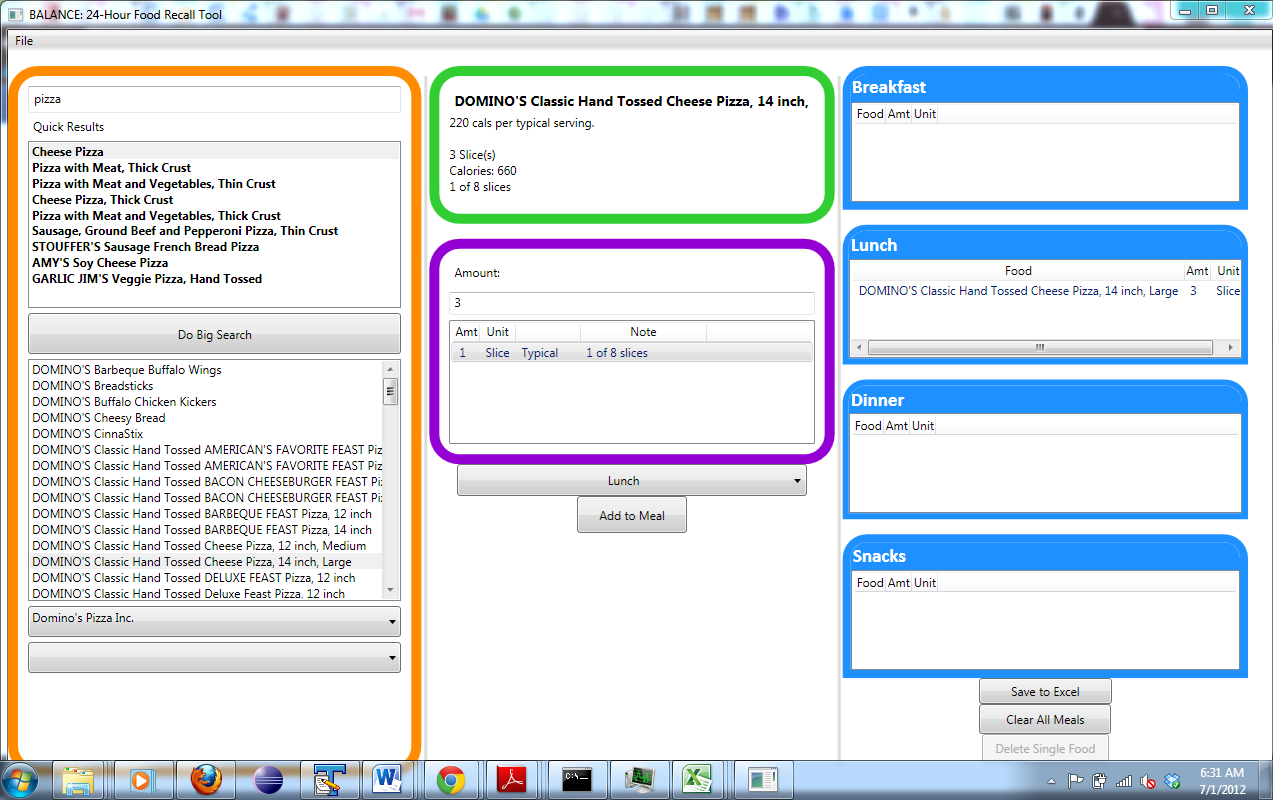
\includegraphics[ width =5.5in ]{./images/cont1/fig12}}

\caption{Software to support the 24-hr recall using the same database and queries as the mobile software.  }
\label{fig:fig12}

\end{center}
\end{figure}

The recall software is pictured in \ref{fig:fig12}. The recall administrator searches for the food in the left pane. The `Quick Results' at the top displays the same foods that the BALANCE mobile user would initially see when searching for a food. The bottom pane allows the administrator to probe about specific manufacturers. The middle pane provides details on a single food and allows amounts to be specified. The right pane shows the foods that have been entered for each meal. The final recall data can be exported to Excel for analysis. 

\subsection{Metrics}
For the evaluation of the focus group-based iterative design process, we defined one measure of interest to be the time between when a food was eaten and when it was entered into the food diary. We found this to be problematic for two reasons: First, participants reported preferring to make entries at the end of the day, regardless of when they ate; second, it relied on participants correctly entering the time that a food was eaten as part of the food entry. As reported in \citet{hughes_balance_2010}, not enough participants modified the time that a food was eaten to make this a useful measure. This led us to consider if other measures could better reflect use of the food diary. Therefore, a secondary goal of this validation phase was to collect data to generate multiple metrics. 

The HCI and Persuasive Technology research communities recognize the potential value of metrics that reflect more details about the use of food diaries. Researchers working in the space of health and wellness have long acknowledged that actual behavior change cannot be the primary measure of success for evaluating tools to help support behavior change \citep{klasnja_how_2011}. Early prototypes and investigations into the space need other measures to indicate whether the tool is developing in the right direction or not. In this vein, researchers are increasingly focusing on \textit{indicators of engagement}, which, loosely defined, are metrics that reflect how engaged an individual is with a particular tool. The reasoning is that the higher the level of engagement (and the more sustained the engagement), the greater the chance for behavior change. However, the usefulness of different indicators of engagement is unclear. 

Additional details about the BALANCE validation study are reported in Snively (\citep{snively_balance_2010}). There, in regards to the food diary, she reports on the overall calories entered into the food diary, the calories reported on the food recall, and analyzes discrepancies. She reports feedback on the usability of the software, but does not report on metrics that indicate patterns of use of the BALANCE food diary. 

In this section, I describe the data that was collected, the metrics that were generated, and report on how well they reflect how the software was used. I also address how these metrics could help interpret the final validation results, which identified a discrepancy between calories entered into the food diary and calories determined via the 24-hr recall. 

\subsubsection{Overview}
As described in Chapter \ref{cha:relatedWork}, previous work reports summary measures of food diary use. These reported measures are usually means reflecting the entire study period. In the rest of this section, I provide more detail, but here I present a quick overview. 

Table \ref{tab:balMetricMeans} reports the means for the four metrics. Days 1-4 reflect active participation in the study. I also include data about Day 5. We found relevant and potentially significant use of the food diary on Day 5, which is technically outside of the study period. 

% Table generated by Excel2LaTeX from sheet 'cont1_meanStartsPerDay'
\begin{table}[htbp]
  \centering
  \caption{Means per participant, per day.}
    \begin{tabular}{lll}
    \toprule
          & Days 1-4 & Days 1-5 \\
    \midrule
    Number of times the software is started & 2.7   & 2.3 \\
    Number of entries created & 9.5   & 8.42 \\
    Number of foods eaten & 9.67  & 8.2 \\
    Number of record edits & 3.02  & 2.97 \\
    \bottomrule
    \end{tabular}%
  \label{tab:balMetricMeans}%
\end{table}%

The means presented above provide a summary understanding of the use of the BALANCE food diary. To further characterize patterns of use over time, each study day is broken into six 4-hr periods, summarized in Table \ref{tab:studyDayTimePeriods}. No distinction is made between weekends and weekdays. These time periods are used for the more detailed analysis in this section. 

% Table generated by Excel2LaTeX from sheet 'Sheet1'
\begin{table}[htbp]
  \centering
  \caption{Add caption}
    \begin{tabular}{ll}
    \toprule
    \textbf{Time frame} & \textbf{Hours} \\
    \midrule
    Early Morning & 12am-4am \\
    Morning & 4am-8am \\
    Late Morning & 8am-12pm \\
    Afternoon & 12pm-4pm \\
    Evening & 4pm-8pm \\
    Night & 8pm-12am \\
    \bottomrule
    \end{tabular}%
  \label{tab:studyDayTimePeriods}%
\end{table}%


\subsubsection{App starts over time}
We start by looking at how often the BALANCE app is started over the course of the study period. Starting the app usually indicates that the user is thinking about the app. In the case of the BALANCE software, starting the app could reflect that the user just ate and is planning to make an entry; is planning to eat and looking up an CHIP values; is glancing at the visualization to assess progress in the middle of the day; or is planning to enter a forgotten entry from earlier in the day. 

As discussed in Chapter \ref{cha:relatedWork}, some researchers report the mean number of times the food diary software was started each day. We calculated this by counting the number of times the software was started over the four days of the study, then dividing by four (the number of days in the study). This results in a mean number of app starts per day in the study period of 2.70. However, we saw that many participants (18) started the software and made entries on the fifth day after the study started. The mean number of app starts over five days is 2.3. 

Figure \ref{fig:chartMeanStartsPerDay} shows the mean number of app starts for each day of the study, including Day 5. The standard deviation is shown as error bars. As expected, the amount of use declines over each day. The low mean on Day 2 reflects that participants were not required to enter their food intake that day. 

\begin{figure}[ tbh ]
\begin{center}

\setlength\fboxsep{0pt}
\setlength\fboxrule{0.5pt}
\fbox{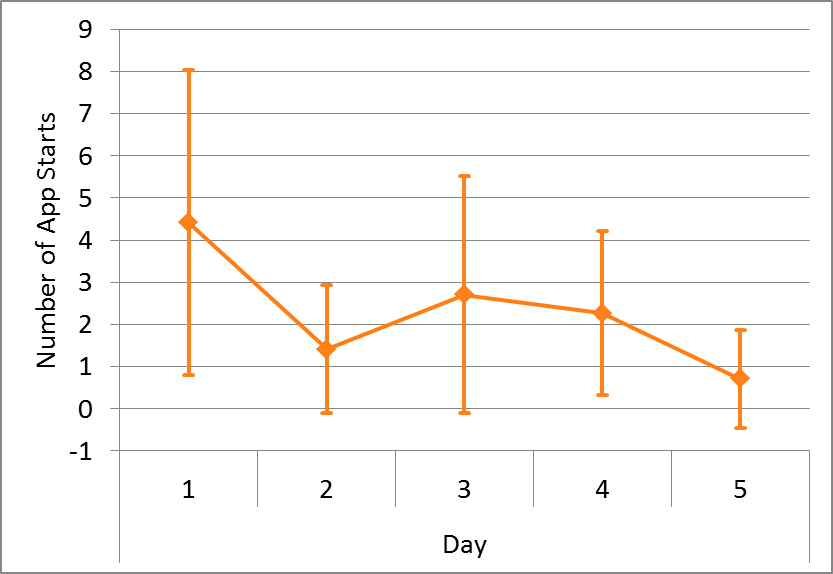
\includegraphics[ width =10cm ]{./images/cont1/chart_meanStarts}}

\caption{Mean app starts for each day. }
\label{fig:chartMeanStartsPerDay}

\end{center}
\end{figure}

One concern we have about reporting the mean number of app starts is its summarizing nature. The mean and standard deviation reflect how much the software was used on each day. However, the BALANCE project is concerned with the distribution of app use throughout a day. The mean does not reflect the relationship between how many times the app was started and how many meals or eating episodes were captured. Participants could start the app repeatedly to enter a single meal, start the app one time for each meal, or start the app one time to enter multiple meals.  

To address this, we calculated how many times the app was started in every 4-hr time period after the start of the study (midnight of Day 1), per participant. The data revealed that some people started the app in multiple time periods; some only started the app within one time period; and some people never started the app. Figure \ref{fig:chart13} reflects how many people reflected each pattern of use. 

\begin{figure}[ tb ]
\begin{center}

\setlength\fboxsep{0pt}
\setlength\fboxrule{0.5pt}
\fbox{\includegraphics[ width =10cm ]{./images/cont1/chart13}}

\caption{App start patterns over the days }
\label{fig:chart13}

\end{center}
\end{figure}


If everyone used the software the way we intended them to, the Figure \ref{fig:chart13} would show 34 people starting the app in multiple time periods (orange) on Days 1, 3, and 4. However, this is not what we see. Consistent with the mean app starts per day, the number of people starting the app in multiple time periods decreased on Days 3 and 4. Inspection of the raw data revealed that 11 people displayed the desired pattern, which indicated that they used the app as requested. 13 people had at least one day (of days 1, 3, or 4) where they did not start the app at all. Five people had two days when they did not start the app at all. Two people started the app one time/day for all four days.

One problem with this calculation is that not starting the app does not always indicate a participant was not using the app consistently throughout the study. Two participants started the app zero times throughout the study period, but still had valid entries. This can be explained that participants treated the phone as a special device used only to enter their food. Since participants were asked to carry a separate device rather than use their personal phone, they were not using the device for anything else. This meant they likely had no reason to ``quit'' and re-start the app. 

\textbf{What does this mean for the validation discrepancy?} This data indicate that for the most part, participants were starting the application periodically through the day. This meant that the discrepancy is probably not due to people forgetting about the application. 

\subsubsection{When entries are made}
Figure \ref{fig:numPeopleEntriesOverTime} shows how many participants created entries during each specified time period. With this population, it was fairly unpopular to make entries in the early morning and morning, while the late morning, afternoon and evening were the most popular times to make entries. 


\begin{figure}[ t ]
\begin{center}

\setlength\fboxsep{0pt}
\setlength\fboxrule{0.5pt}
\fbox{\includegraphics[ width =10cm ]{./images/cont1/chart14}}

\caption{Number of people who made entries in a given time period.}
\label{fig:numPeopleEntriesOverTime}

\end{center}
\end{figure}

\subsubsection{Entry creation time}
This data is generated by counting the number of entries created in a given time period, over the course of the study. This only counts when a record was created in that time period. It does not account for when a food was entered for a different time. This better reflects the pattern of entries that are made throughout the study period, specifically when people are thinking about or using the application. It does not always reflect when people actually ate. 
 
\begin{figure}[ t ]
\begin{center}

\setlength\fboxsep{0pt}
\setlength\fboxrule{0.5pt}
\fbox{\includegraphics[ width =10cm ]{./images/cont1/chart15}}

\caption{Number of entries over time}
\label{fig:chart15}

\end{center}
\end{figure}

This chart shows a sum of all the entries entered during a particular time period each day. While the above chart showed the number of participants who made entries in that time period, this indicates how many entries those participants actually made. 

\textbf{What does this mean for the validation discrepancy?} Reviewing the charts, we see that Day 1 has more people who made more entries earlier in the day. In contrast, on Days 3 and 4 participants made entries primarily in the second half of the day, creating more entries in the second half of the day than in the first half of the day. This indicates that participants were probably entering their food closer to the time that they ate it on Day 1. This implies that the Day 1 entries probably more closely reflects what they actually ate. 

\subsubsection{Food eaten time}

\begin{figure}[ tbh ]
\begin{center}

\setlength\fboxsep{0pt}
\setlength\fboxrule{0.5pt}
\fbox{\includegraphics[ width =10cm ]{./images/cont1/chart16}}

\caption{Number of entries eaten over time.}
\label{fig:chart16}

\end{center}
\end{figure}

Figure \ref{fig:chart16} shows how many valid food entries were reported as being eaten in the given time period, independent of when they were created. 


A comparison of \ref{fig:chart15} and \ref{fig:chart16} indicates that participants likely made entries in the second half of the day capturing food that they ate in the first half of the day. 

\textbf{What does this mean for the validation discrepancy? }Similar to the entry creation time, usage on days 3 and 4 indicate patterns that correlate to greater error between what was eaten and what was entered. This appears less extreme on day 1, so again, the entries on day 1 probably more closely match what was actually eaten. 


\begin{figure}[ t ]
\begin{center}

\setlength\fboxsep{0pt}
\setlength\fboxrule{0.5pt}
\fbox{\includegraphics[ width =5in ]{./images/cont1/chart15_b}}

\caption{Number of entries entered and created over time}
\label{fig:eatenVersusCreated}

\end{center}
\end{figure}

\begin{figure}[ t ]
\begin{center}

\setlength\fboxsep{0pt}
\setlength\fboxrule{0.5pt}
\fbox{\includegraphics[ width =5in ]{./images/cont1/chart_meanEntriesEaten}}

\caption{Number of entries entered and created over time}
\label{fig:eatenVersusCreatedperDay}

\end{center}
\end{figure}

\subsubsection{Comparing entry creation and food eaten time}
Figure \ref{fig:eatenVersusCreated} shows a comparison of the number of records created versus food entries eaten over time. Day 2 shows that there were more entries created than eaten. Since Day 2 was the day participants did not need to make entries, this probably indicates that participants were filling in entries for Day 1, where there are more entries eaten than created. In Days 3, the eaten and created peaks are offset, again indicating that participants probably used the food diary at night to make entries for food eaten in the late morning. Day 4 also shows that morning, late morning and afternoon had more food entries eaten than entered. In this case, they appear to have been created in the afternoon of Day 5. 

\textbf{What does this mean for the validation discrepancy? }Similar to the entry creation time, usage on days 3 and 4 indicate patterns that correlate to greater error between what was eaten and what was entered. This appears less extreme on day 1, so again, the entries on day 1 probably more closely match what was actually eaten. 

\subsubsection{Entry edits}

\begin{figure}[ t ]
\begin{center}

\setlength\fboxsep{0pt}
\setlength\fboxrule{0.5pt}
\fbox{\includegraphics[ width =10cm ]{./images/cont1/chart17}}

\caption{Number of edits over time}
\label{fig:chart17}

\end{center}
\end{figure}


One indicator that users are becoming more familiar and comfortable with a piece of software or an interface is how many errors they make. In this study, the best indication we have for the number of errors people make throughout the whole study is how many edits they make.
 
The mean number of edits made by participants over the entire study is 13.559, with a standard deviation of 8.33. 

Figure \ref{fig:chart17} shows how many edits were made each day of the study, by all of the participants. The decrease in edits over time could indicate that participants were becoming more comfortable with the software, and making fewer errors in their entries. The increase on day 5 could reflect participants checking their entries to prepare for the completion of the study. 

\textbf{What does this mean for the validation discrepancy? }The high number of edits on day 1 could indicate that participants were being conscientious about ensuring that the records were correct. 

\subsubsection{Number Of Combos/Favorites And Their Use}
One of the features asked for many times in the focus groups the ability to save and use favorite foods, combinations, and recipes. In the validation study, 2 participants created 2 combos total, and used one of the combinations 2 times in their diary. 


\subsubsection{Putting it all together }
So far, this section has described metrics that attempt to characterize the use of the food diary over the duration of the study. Now, I will show how the overviews reflect the usage patterns of an individual participant. I will show the details of two participant. The first has the distinction of being one of the participants who did not ever start or quit the application, but otherwise used the food diary as expected. The second participant showed a slightly different pattern of use. 

\begin{figure}[ tb ]
\begin{center}

\setlength\fboxsep{0pt}
\setlength\fboxrule{0.5pt}
\fbox{\includegraphics[ width =5.5in ]{./images/cont1/chart18}}

\caption{All measures, Participant 101}
\label{fig:chart18}

\end{center}
\end{figure}

Figure \ref{fig:chart18} shows all of the measures for Participant 101. This participant showed a decent amount of food diary activity for Days 1, 3, and 4, which is what is expected for this study. However, this is one of the participants who left the software running the entire time. Therefore, no app starts were detected.  On Day 1, in the morning, more foods were eaten than entered, but in the afternoon more foods were entered than eaten. This shows that the participant entered some of the food eaten in the morning, but later in the day went back and added some more entries. On Day 3, the participant was consistent about entering entries when the food was eaten. On Day 4, many more entries were eaten in the afternoon and evening than were entered. On Day 5, some more entries were made, which explains that the participant went back and filled those entries in. 

\begin{figure}[ t ]
\begin{center}

\setlength\fboxsep{0pt}
\setlength\fboxrule{0.5pt}
\fbox{\includegraphics[ width =5.5in ]{./images/cont1/chart19}}

\caption{Patterns of use, ppt120}
\label{fig:chart19}

\end{center}
\end{figure}

Figure \ref{fig:chart19} shows the details for Participant 120. Overall, this participant shows a more consistent interaction with the food diary. The app is started for each time period that we have data. For the most part, entries are entered at the time of eating, with a few edits. Day 1 shows more interaction with the software, which is consistent with a period of adjusting to it. Also, while there are many edits the first day, there are fewer edits in later days, which could indicate a greater familiarity with the software. Starting the app on Day 6 could reflect the participant starting the software to show the study administrator. Day 3 shows that the participant created more entries early in the day, but ate more entries later in the day. This could indicate a planning behavior on behalf of the participant. 

\subsection{Discussion }
In this section, we reviewed metrics that reflected how participants used the food diary in the BALANCE validation. We looked at how and when participants started the food diary app, created entries, reported food as being eaten, and made edits. Participants appeared to start the app more and make more edits on the first day of the study, but the number of entries created and foods eaten were consistent on all three days of the study. This reflects that participants were becoming familiar with the software on the first day. 

The measures show interaction with the software on Days 2 and 5. Day 2 is when participants were not supposed to enter their food, while Day 5 was the day after the study period. The interaction on those days showed that some participants were filling in earlier entries. We also saw that with participant 120, some participants likely used the software to plan ahead, by making entries that reflect being eaten later in the day. 

For this validation phase of the BALANCE study, we chose to present a more detailed treatment of the collected measures due to our experience with the focus group evaluation. In the focus group evaluation, the measure we were interested in was the time between when a food was eaten and when the food entry was created. This measure was not meaningful because too few participants entered the food eaten time when creating the food entries. However, in this validation study, we see evidence that participants did modify food eaten times. There are two potential explanations for this discrepancy. First is that the software was modified throughout the focus group evaluations, and before this final validation. The process to modify a food eaten time may have improved enough to make it easier for participants to modify the entries to reflect the time it was actually eaten. Second, the small sample sizes in the focus groups could impact the effectiveness of the measure. While the validation study does show that participants modified food entries, we also see that some participants probably did not modify the food eaten time. One or two people in each focus group not modifying the food eaten time would impact the quality of that data. 

Previous research has identified factors that increase error in food diaries that people create. In the BALANCE validation study, we identified a discrepancy between what they entered and what was reported in a 24-hr recall. Previous work comparing food entries in an electronic food diary to a 24-hr recall found no significant difference (\citep{glanz_improving_2006}), but one difference between that study and this is that the 24-hr recall was performed a few days into a long-term study, rather than on the first day of a 3-day study. This raises two questions: whether participants were not as familiar with the software and device on the first day, and if the discrepancy may improve if the comparison was performed on the third or fourth day. However, the patterns of use in this study reveal that the Day 1 of the study was probably the most complete food diary data. 

\section{Overall Discussion}
The BALANCE project provides a rich dataset for us to begin understanding some of the challenges that people encounter when trying to self-monitor their food intake on mobile phones. Over the course of our four studies, almost 50 people used the food diary for 3 days and provided detailed feedback. We collected usage metrics of 34 of those participants. These metrics helped us to better understand some of the patterns of use. All of this data also helped us to better understand how our metrics and methodology impacted the evaluation outcomes. I further elaborate on specific themes below. 

\textbf{Historical Context. } The changing technical capabilities of mobile phones were an issue for this project. The BALANCE project began in 2008. Nokia N80s, considered state-of-the-art at the time, were the first devices running the prototype software. These were soon replaced by Nokia N95s. N95s had a larger screens and better technical capabilities overall. The focus group evaluation started in early spring 2009 and finished in late fall of 2009. The validation phase began in spring 2010 and finished in the fall of 2010.

At the beginning of the project, PDAs had been commercially available for more than 10 years, but smartphones were still considered high-end, early adopter technology. Up until that point, both smartphones and PDAs were increasing in capability, but consumers had to choose between the two. However, smartphones were just beginning to merge with PDAs. When this happened, smartphones with touch screens became accessible for consumers. 

Altogether, when we began this project, most people were not using their phone for much more than a basic phone. This was the case even for people with more capable smartphones or PDAs. However, they increasingly aware of the notion of using ``apps'' on a phone. 

\textbf{Fast-changing Technology. } The phone we provided for participants in the focus groups (the WinMobile-based HTC Fuze) was considered `very cool'. One notable comment from a participant was that her teenage son thought she was lucky to be able to use that phone. However, by the end of the project, comments from participants included ``the phone is so clunky and slow''. Indeed, one challenge we have going forward is that it is not likely to be the same phone model as the existing research that has been done. Changing technology platforms throughout a research project introduces challenges for the researchers, but not keeping up with consumer expectations could impact their impressions and feedback of the tool. 

\textbf{Personal Devices.} Administering studies using mobile phones requires researchers to choose whether participants should carry a dedicated study device or if the study software should be installed on a participant's personal device.    \citet{consolvo_conducting_2007} indicate the latter case may be preferable because the participants are familiar with the device and have all of their contact and other personal data on it, therefore may be more likely to use the software on a regular basis. However, study prototypes may be unstable, causing the phone to crash or otherwise interfere with the normal functioning of the phone. In the case of a study-provided device, the participant may be unfamiliar with the device, or have to carry two devices, which may make them less likely to use the software. 

In the BALANCE studies, we chose to provide study-owned devices to the participants to use in addition to their personal phones because of the technical requirements of the project. This could have impacted participant ability to adopt the software readily. The validation study showed evidence that some participants did not start and stop the software as expected. 

\textbf{User Expectations and Research Goals.} 
We had two interim goals as part of the BALANCE project. One goal was to incorporate user feedback to inform the design of the BALANCE software. The other goal was to use the software to collect data to evaluate hypotheses about how the technology supports people tracking their energy intake and expenditure. 


\textbf{User Expectations. }
Researchers developing mobile applications face similar conflicting priorities as developers in a commercial setting.  Putting software into the hands of real users is the best way to help the researcher determine how the software will really be used, what its best and worst features are, and what bugs require repair most urgently. Yet at the same time, users are often intolerant of buggy software and unable to report much more than "it didn't work" as a bug report. As a compromise, we use an iterative approach,  incorporating feedback after each version, and informing testers to the greatest extent possible about the status of the software and procedures for bug reporting.


\textbf{Database. }The food database had a huge impact on the overall design and implementation of the BALANCE software. There was a tension between needing a database that was big enough to have all the foods that many different people may encounter, but small enough to make it quick and easy to navigate. The information architecture of the database was important too-food groups and categories that are meaningful to experts and professionals may not be obvious to consumers. This is consistent with reports of the importance of high literacy abilities to navigate food and nutrition information \citet{rothman_patient_2006}. 

\textbf{Study Duration. }Choosing the duration of the final validation study required evaluating a tradeoff. A shorter duration reduces the burden on the participant. However, a longer duration provides more opportunity for the participant to adapt their routine to incorporate the self-monitoring, while also tailoring the software to reduce the burden. The personal database grows based on what people enter, making it easier to find and enter food. The favorites features also provide a way to minimize interaction time. The three day duration will not merit the time investment required for personalization, and overall will probably not have a large impact on the tracking process. 

The evaluations indicated that people found it challenging to use the BALANCE software to self-monitor food intake in a timely, complete and consistent manner throughout a day. This is consistent with other work that indicated technical malfunction prevented statistically significant results [ref]. Participants reported that the idea of tracking their food intake on their mobile phone was appealing, and offered valuable insight as to how we as designers and researchers may improve the process, particularly by reducing the amount of effort that goes in to the food intake capture. This allows us to raise the question of whether people will be able to enter food intake on a consistent basis if we reduce the amount of effort, in terms of time, physical entry (entering text or pushing buttons) and mental activity (how much the user needs to think about the process). This is addressed in the next chapter. 

\section{Summary}
In this chapter, I describe the BALANCE project, focusing primarily on the design and development of the food diary component of the project. I also provide an HCI-oriented evaluation of the use of the BALANCE software by participants in-situ, to better understand the results of the more quantitative, [medical]-oriented evaluation. This evaluation identified that one important barrier to participants creating complete, comprehensive and timely food entries is due to the database. I document the challenges of using a food database on resource-constrained devices such as mobile phones, and [prove that nothing more could be done to improve the database experience with this technology]. The database is challenging to navigate and requires mental effort, particularly in real-world context, in addition to requiring time-consuming text entry. User feedback indicated that people understand the value that dietary self-monitoring could provide, but that the BALANCE food diary required too much time. It also indicated that people might be willing to accept a less detailed accounting of their food intake in exchange for a less challenging and time-intensive collection process. 

 
